%--------------------------------------------%
% Template Beamer for presentations in 		 %
% doctoral courses							 %	
% by bchaihuaque@pucp.pe		             %
% Using Madrid Beamer Template				 %
% version 1.0								 %
% Updated at 18/04/2022						 %
%--------------------------------------------%
\documentclass[aspectratio=169]{beamer}

%%%%%%%%%%%%%% Tema %%%%%%%%%%%%%%%%%%
\mode<presentation>{
	\usetheme{madrid}
}
\usepackage[spanish, english]{babel}
\usepackage[utf8]{inputenc}
\usepackage{graphicx}
\usepackage{xcolor} % change the template's color
\usepackage[utf8]{inputenc} 
\usepackage{booktabs} %% to make tables
% see: https://nhigham.com/2019/11/19/better-latex-tables-with-booktabs/
\usepackage{orcidlink} %% ver como se configura logo orcid: https://tex.stackexchange.com/questions/445563/ieeetran-how-to-include-orcid-in-tex-pdf-with-pdflatex
\usepackage{amsmath} %% formulas matematicas
\usepackage{empheq} %% colocar un box en formula
\usepackage{ragged2e} %% para justificar el texto. Colocarlo en cada frame
\newcommand{\orcid}[1]{\href{https://orcid.org/#1}{\textcolor[HTML]{A6CE39}{\aiOrcid}}}

\definecolor{coolblack}{rgb}{0.0, 0.18, 0.39}
\setbeamercolor{structure}{fg=coolblack}

\institute[]{
	%===========Logos en el medio================%
	%\vspace*{-0.35cm}
	
\includegraphics[width=1.2cm]{figures/consorcio.png}
	\hspace*{0.45cm}~%
	%
\includegraphics[width=4cm]{figures/pucp.png}
	%\vspace*{0.35cm}\\
	
	Escuela de Posgrado - Doctorado en Gestión Estratégica \\
	Curso: Seminario de Temas en Gestión y Desarrollo Estratégico 2}
%%%%%% Título y subtítulo %%%%%%%%%%%%
\title{Cultura en (y alrededor de)  las organizaciones }
\subtitle{El lado simbólico de las organizaciones}

%%%%%%% Autores %%%%%%%%%%%%%%%%%%%%%%
\author{Yazmin Illia \\ Bruno Chaihuaque\orcidlink{0000-0001-5982-8505}}

\begin{document}
	
	%\begin{frame}
	%	\titlepage
	%\end{frame}
	\begin{frame}
	\titlepage 
	
\end{frame}

\begin{frame}
	\frametitle{Outline} 
	\tableofcontents 
\end{frame}
\AtBeginSection[]
{
	\begin{frame}<beamer>{Contenido}
		\tableofcontents[currentsection, currentsubsection]
	\end{frame}
}
% Para mostrar el contenido fantasma para ver avance en el outline
\AtBeginSubsection[]
{
	\begin{frame}<beamer>{Contenido}
		\tableofcontents[currentsection, currentsubsection]
	\end{frame}
}
\addtocounter{framenumber}{-1}% If you don't want them to affect the slide number
	\section{"Concepts of Culture and Organizational Analysis" (Smircich, 1983)}
	\begin{frame}{El concepto de Cultura ¿Cómo abordarlo?}
		\begin{center}
			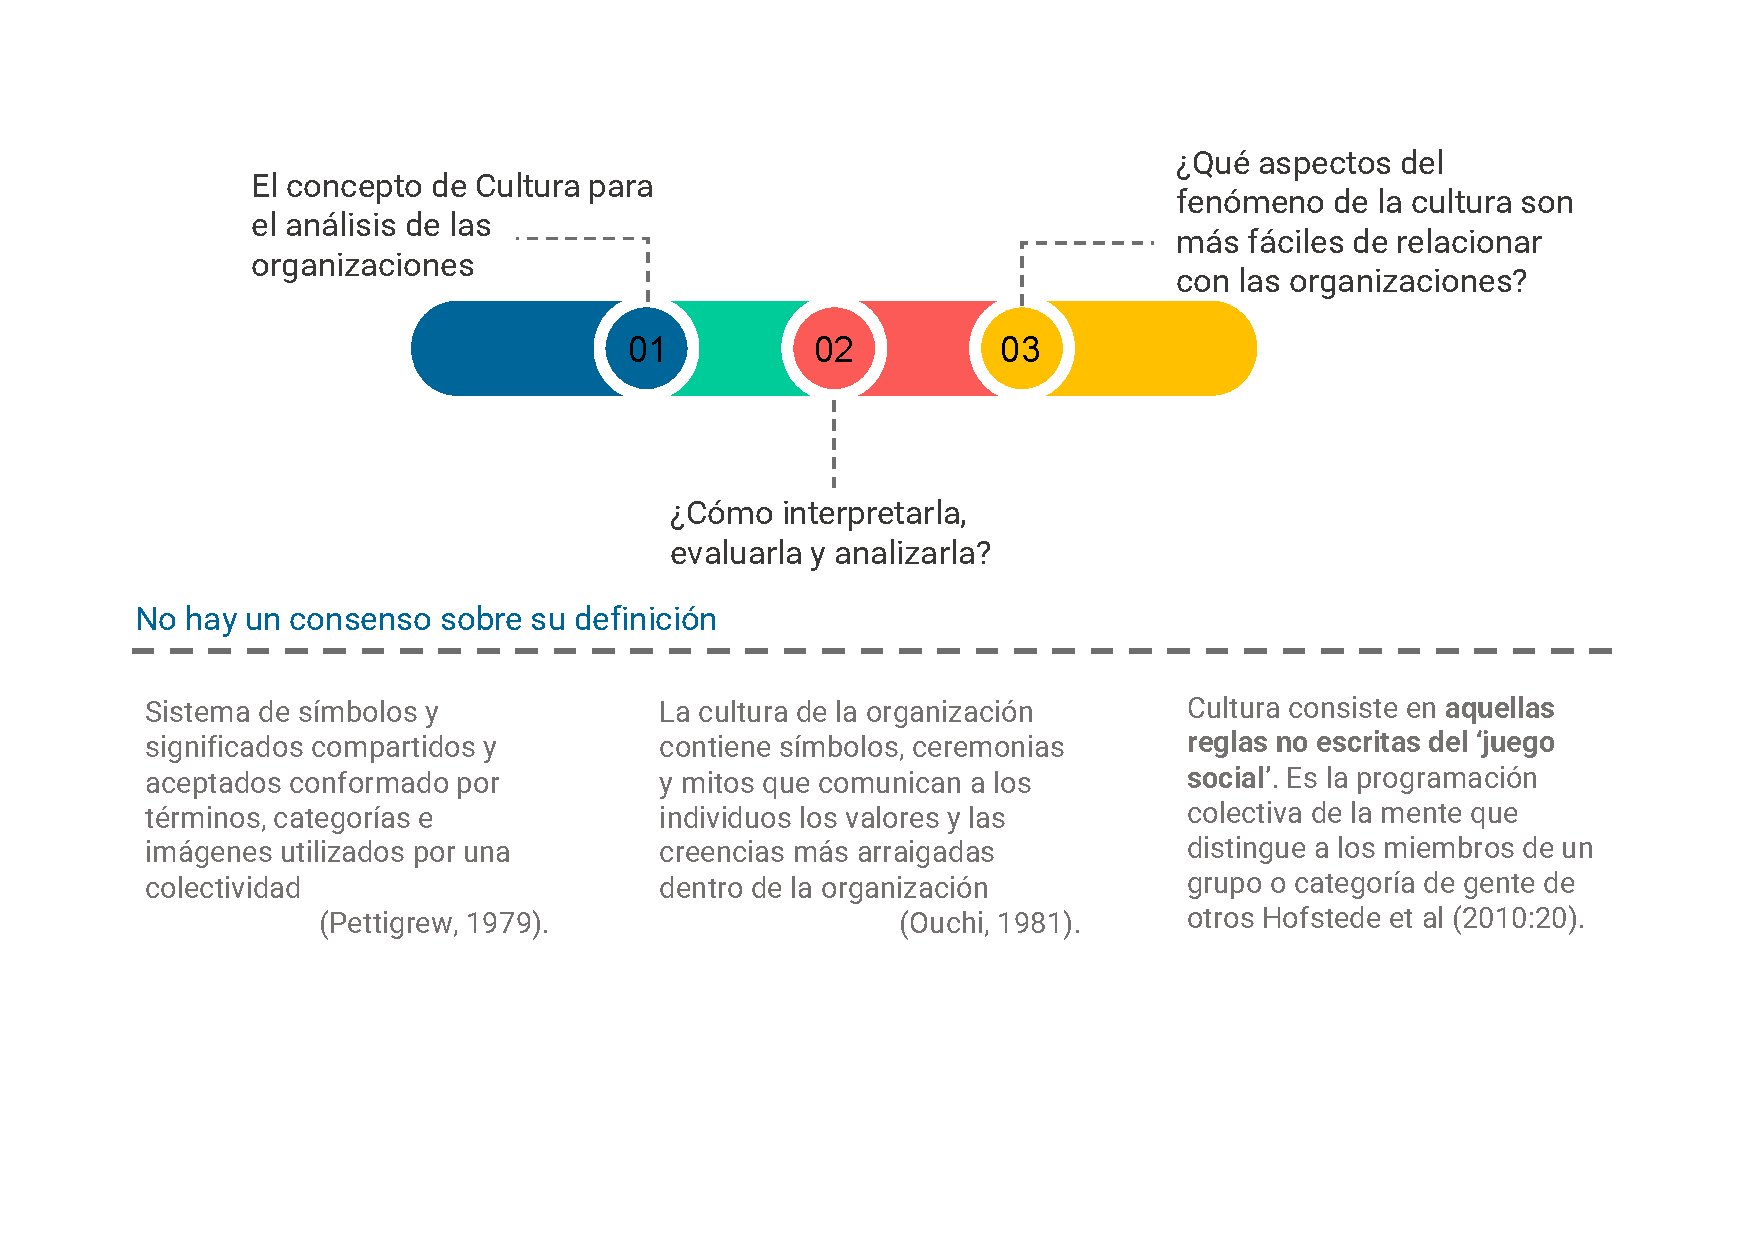
\includegraphics[height=\textheight]{./figures/L1.pdf}
		\end{center}
		
	\end{frame}
	\begin{frame}{El concepto de Cultura ¿Cómo abordarlo?}
		\begin{center}
			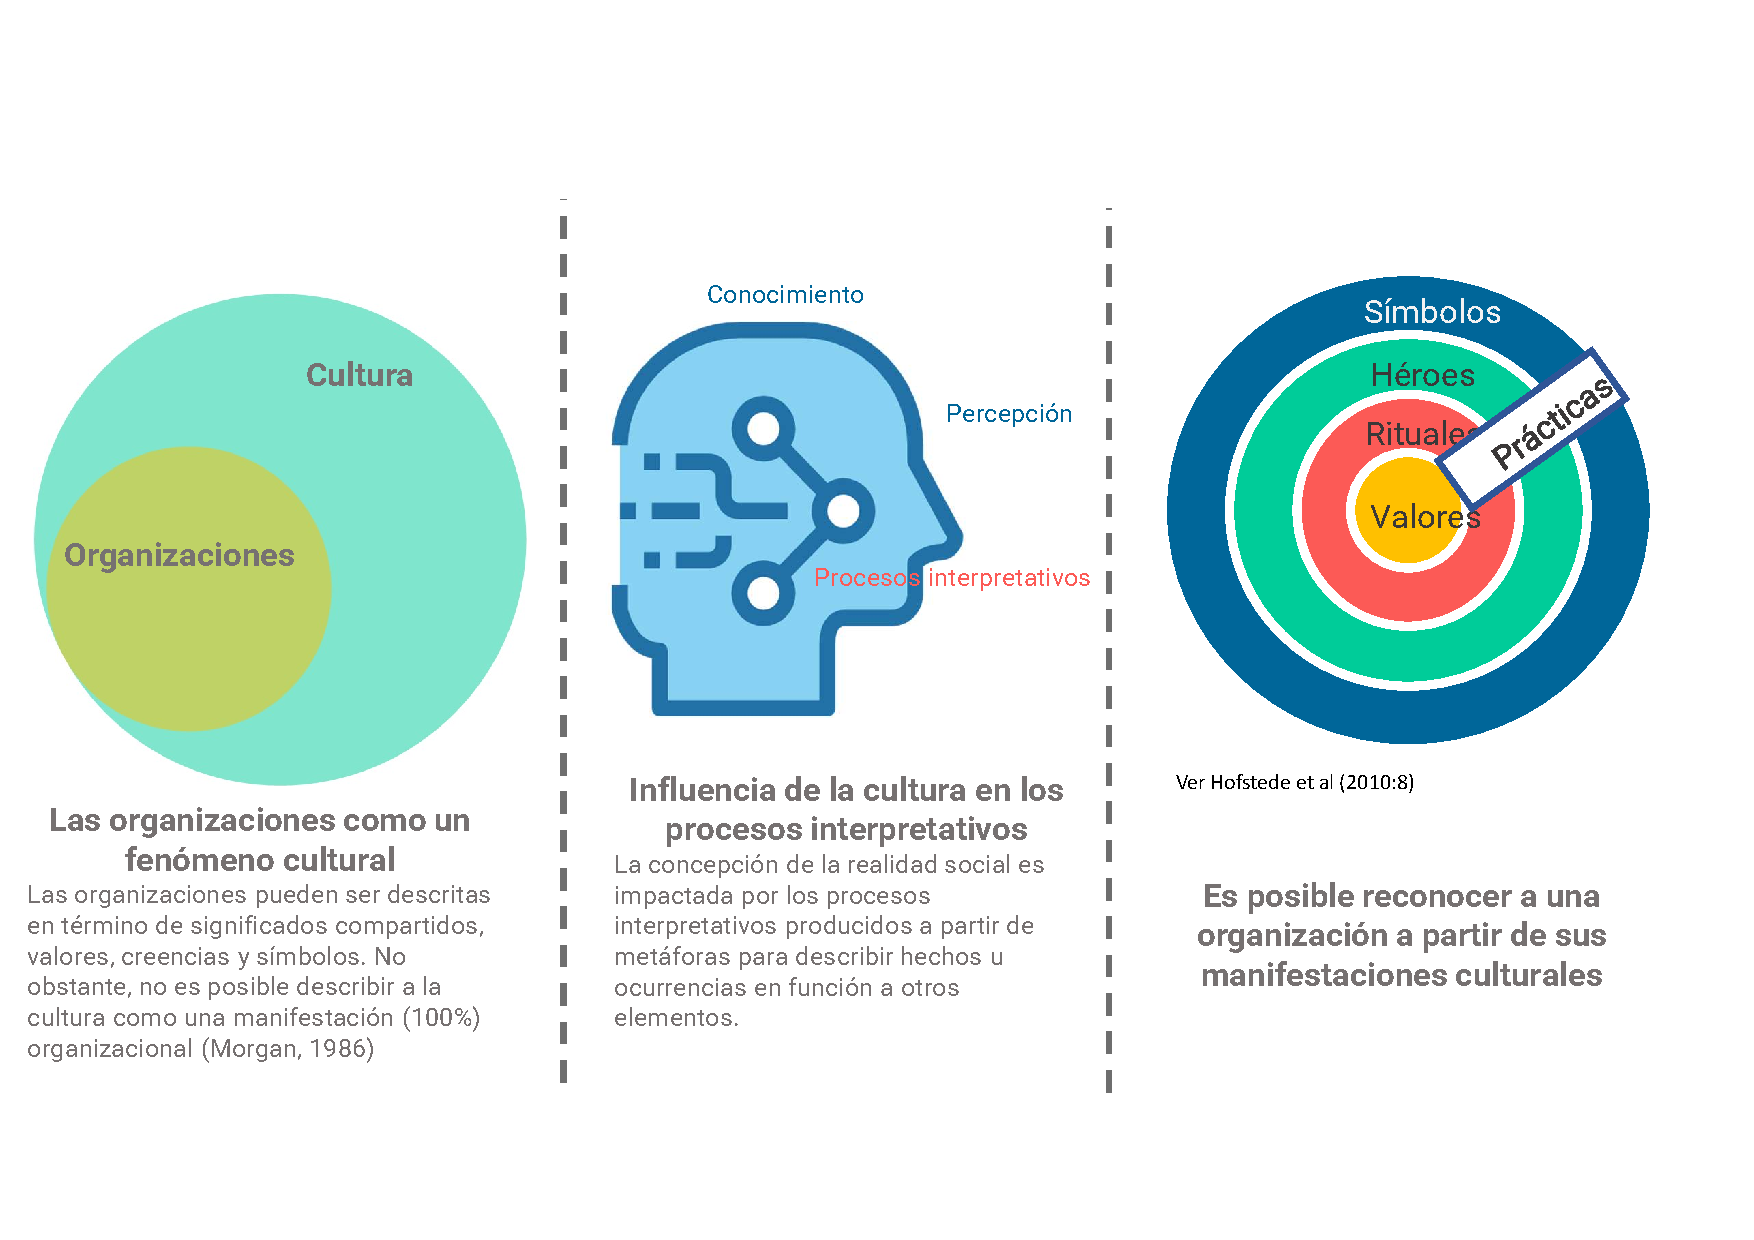
\includegraphics[height=\textheight]{./figures/L2.pdf}
		\end{center}
	\end{frame}
	
	\begin{frame}{Similitudes entre "cultura" y "organización"}
		\begin{center}
			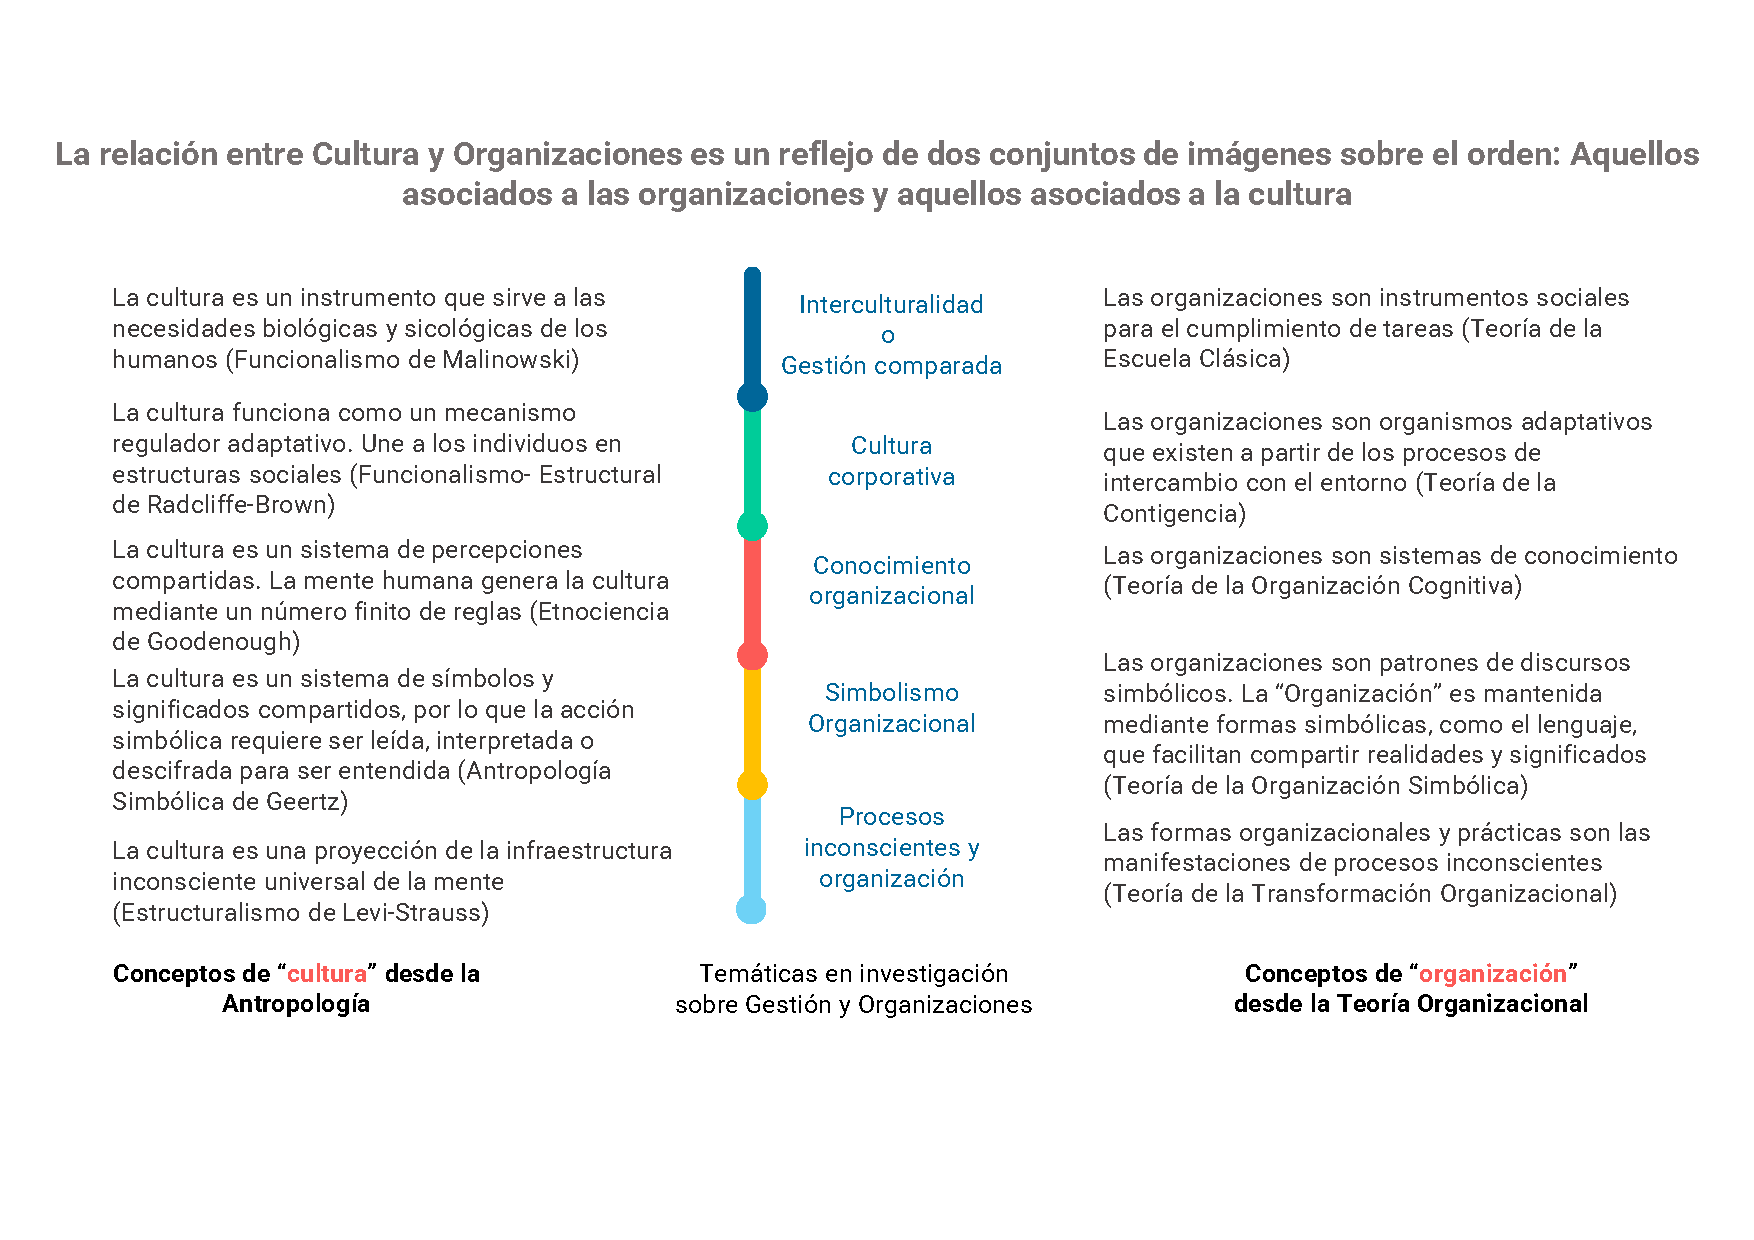
\includegraphics[height=\textheight]{./figures/L3.pdf}
		\end{center}
	\end{frame}

	\begin{frame}{Evolución del Comparative Management y su relación con la Teoría de la Cultura en las Organizaciones}
		\begin{center}
			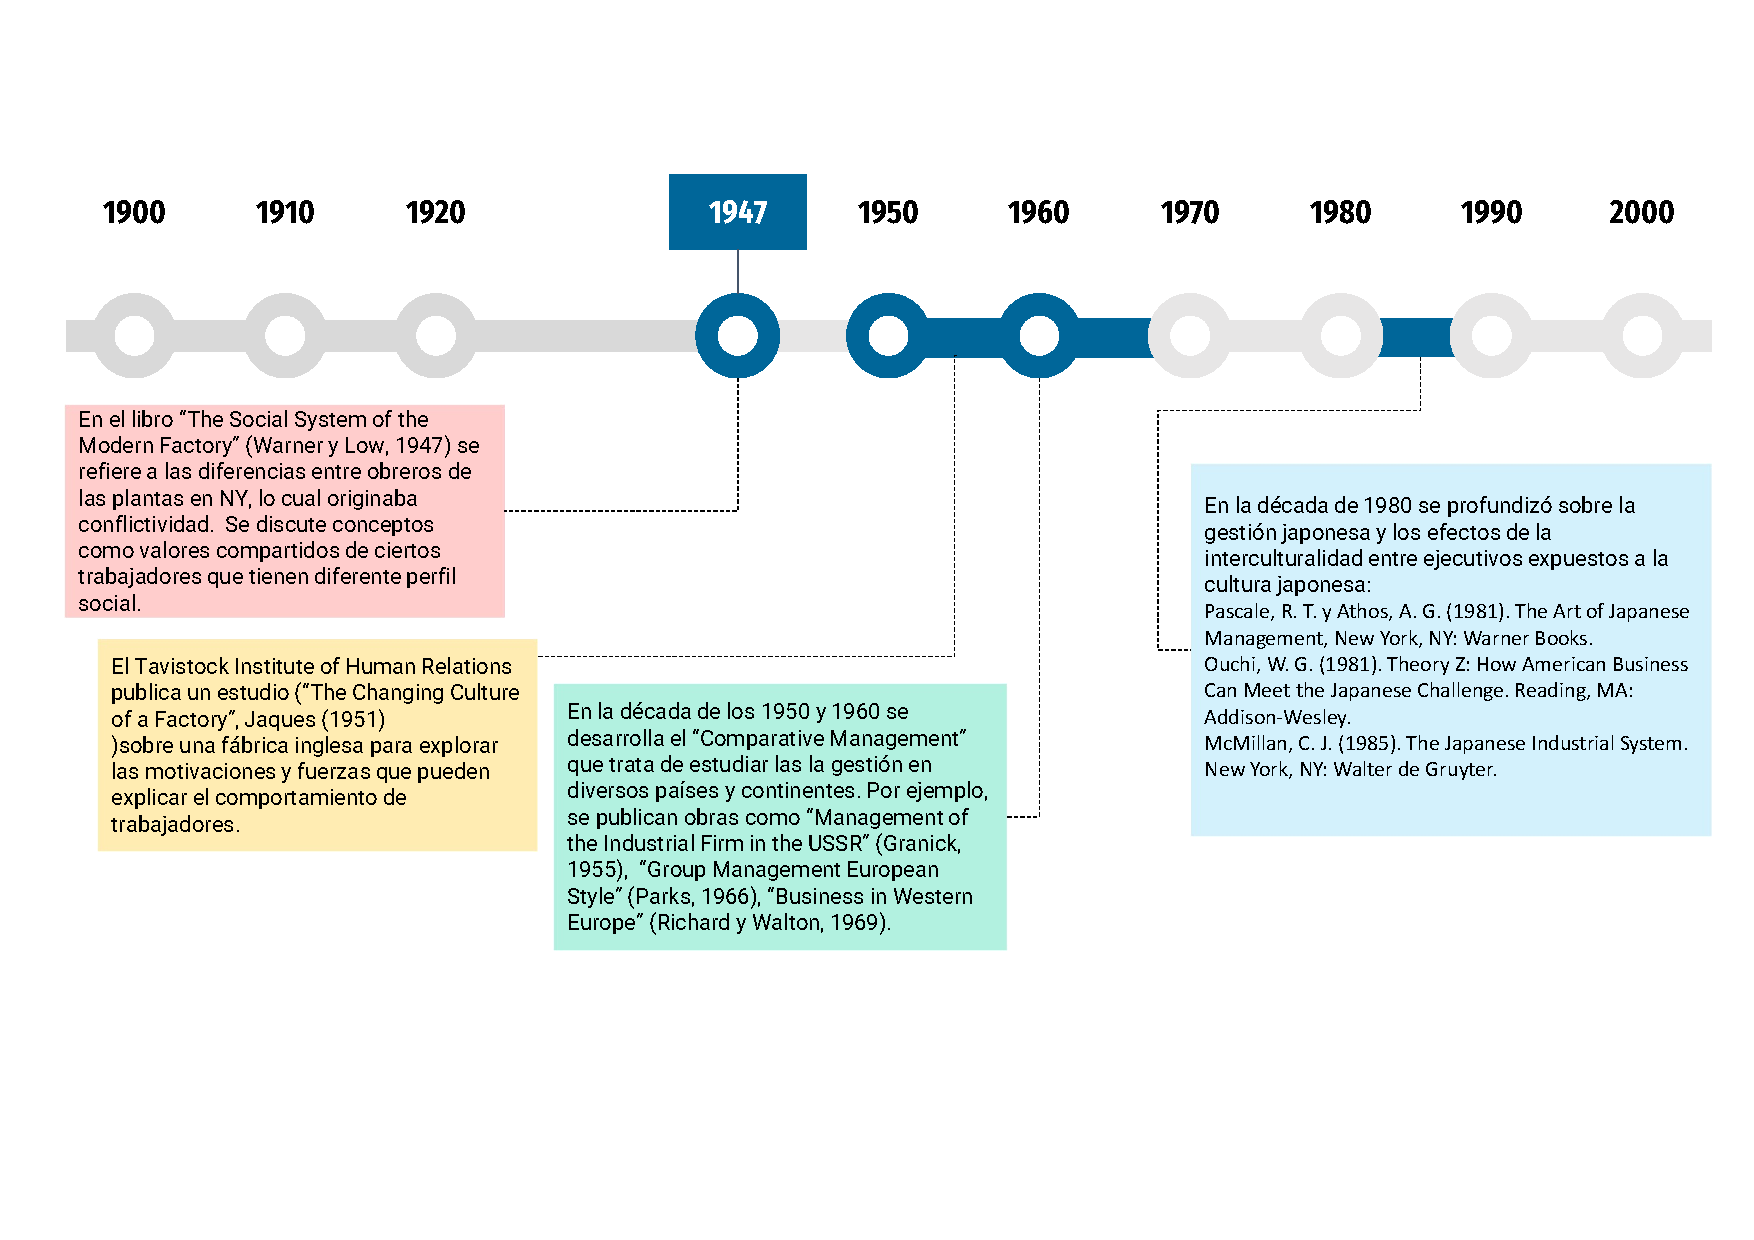
\includegraphics[height=\textheight]{./figures/L4.pdf}
		\end{center}
	\end{frame}

	\begin{frame}{Antecedentes Históricos}
		\begin{enumerate}
			\item Dentro de las ciencias sociales: antropología, la sociología, la psicología social y la economía, investigan el comportamiento del ser humano dentro de distintos grupos sociales y con diferentes funciones, donde la cultura ha estado presente como un resultado de las relaciones interpersonales. 
			
			\item La influencia de la Economía ha sido menor que la de las disciplinas anteriormente descritas, sin embargo los análisis económicos ven en la cultura organizacional una herramienta que puede ser usada para incrementar ganancias. 
			
			\item Ouchi (1982) y Peters y Waterman (1984) buscan en las explicaciones culturales el éxito financiero. Ellos definen excelencia en parte, como un resultado financiero consistente y de alto rendimiento. 
			
			
			
		\end{enumerate}
	\end{frame}
	
	\begin{frame}
		\begin{enumerate}
			\item El concepto de cultura aplicado a la organización se fue gestando desde el aporte de la escuela de administración de las relaciones humanas, a partir de los experimentos desarrollados por Elton Mayo, se empiezan a reconocer los aspectos subjetivos e informales de la realidad organizacional. 
			
			\item Mayo (1972), se interesó por indagar acerca de los factores que inciden en el desempeño del trabajador, llegando a la conclusión que el ambiente del grupo al cual pertenece el individuo incide significativamente en la percepción que éste tiene acerca de los aspectos objetivos de la organización. 
		\end{enumerate}
	\end{frame}
	\begin{frame}{Cultura y "Comparative Management": La Cultura como variable independiente}
		\begin{center}
			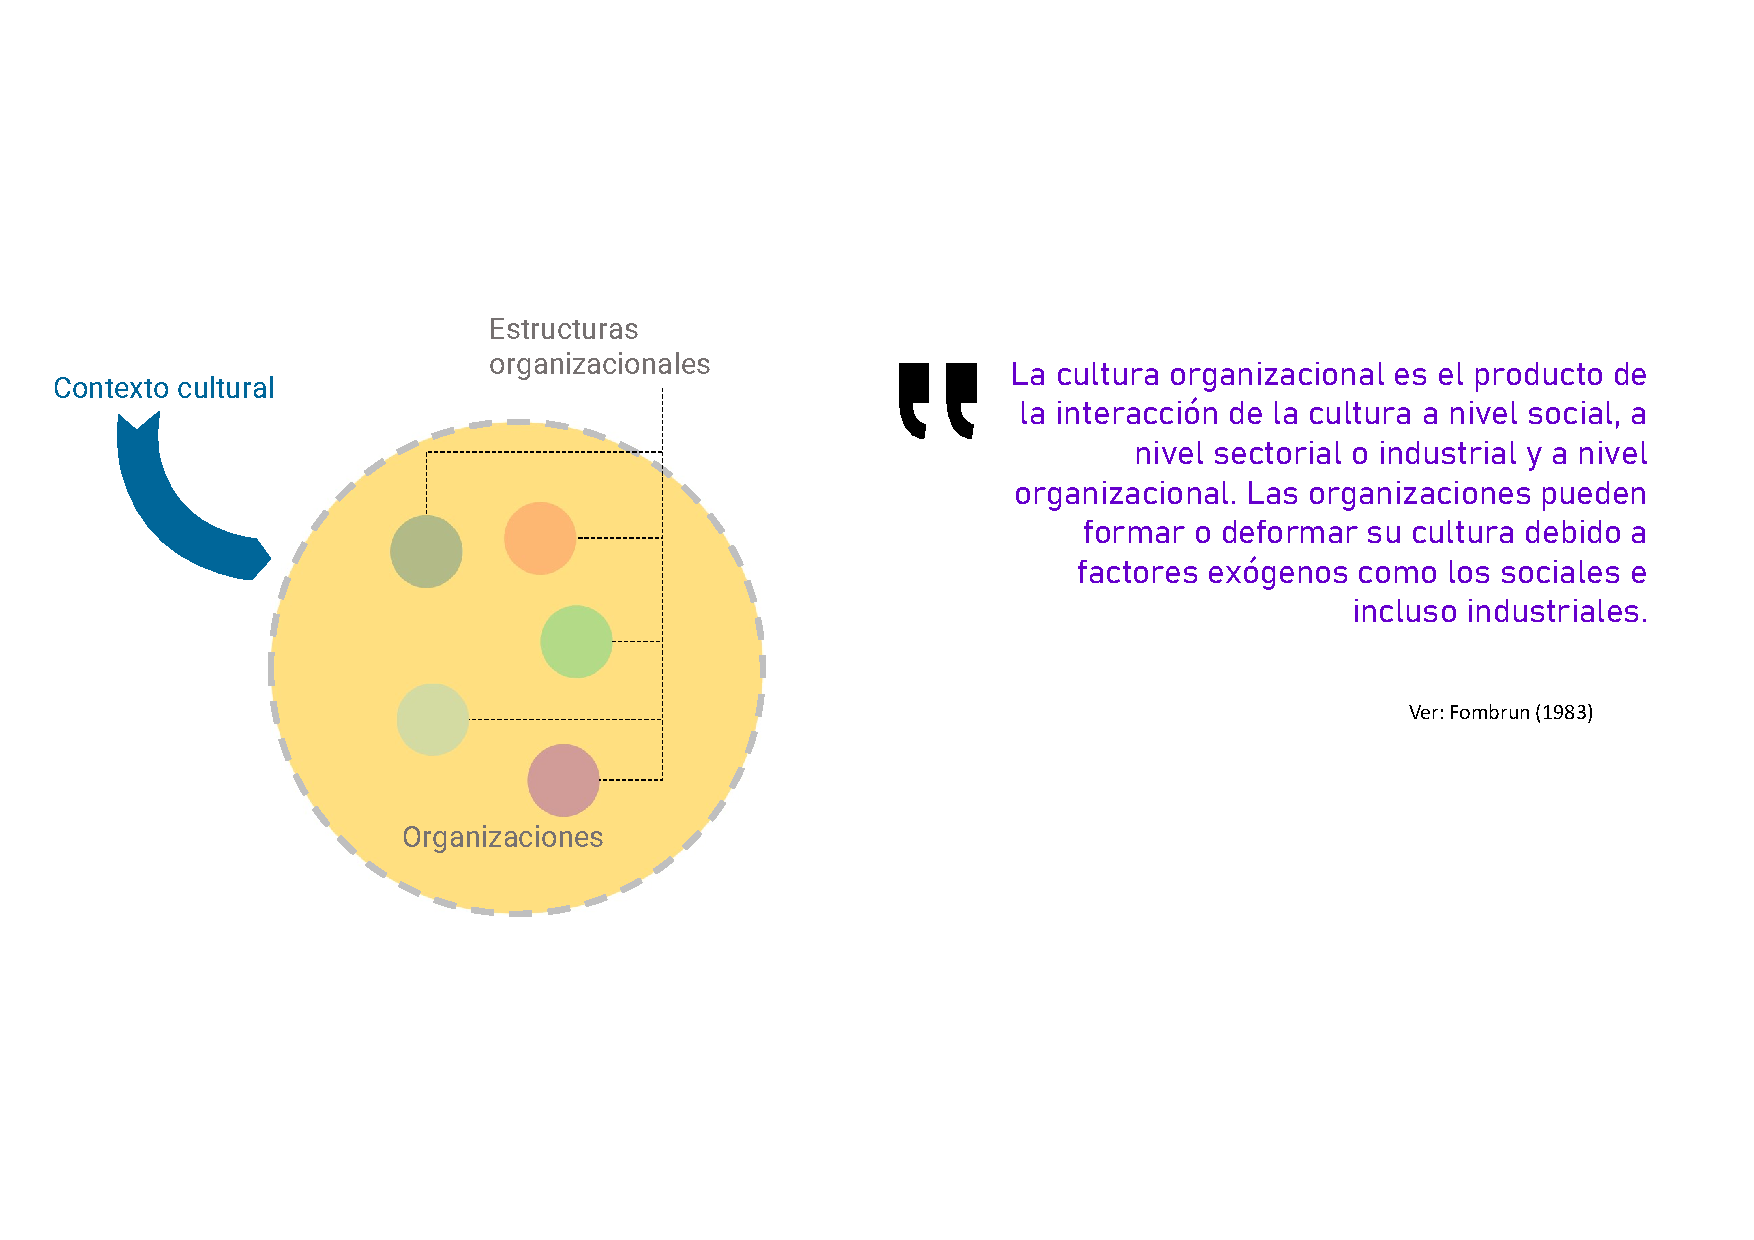
\includegraphics[height=\textheight]{./figures/L5.pdf}
		\end{center}
	\end{frame}

	\begin{frame}{Cultura y "Comparative Management": La Cultura como variable independiente}
		\begin{center}
			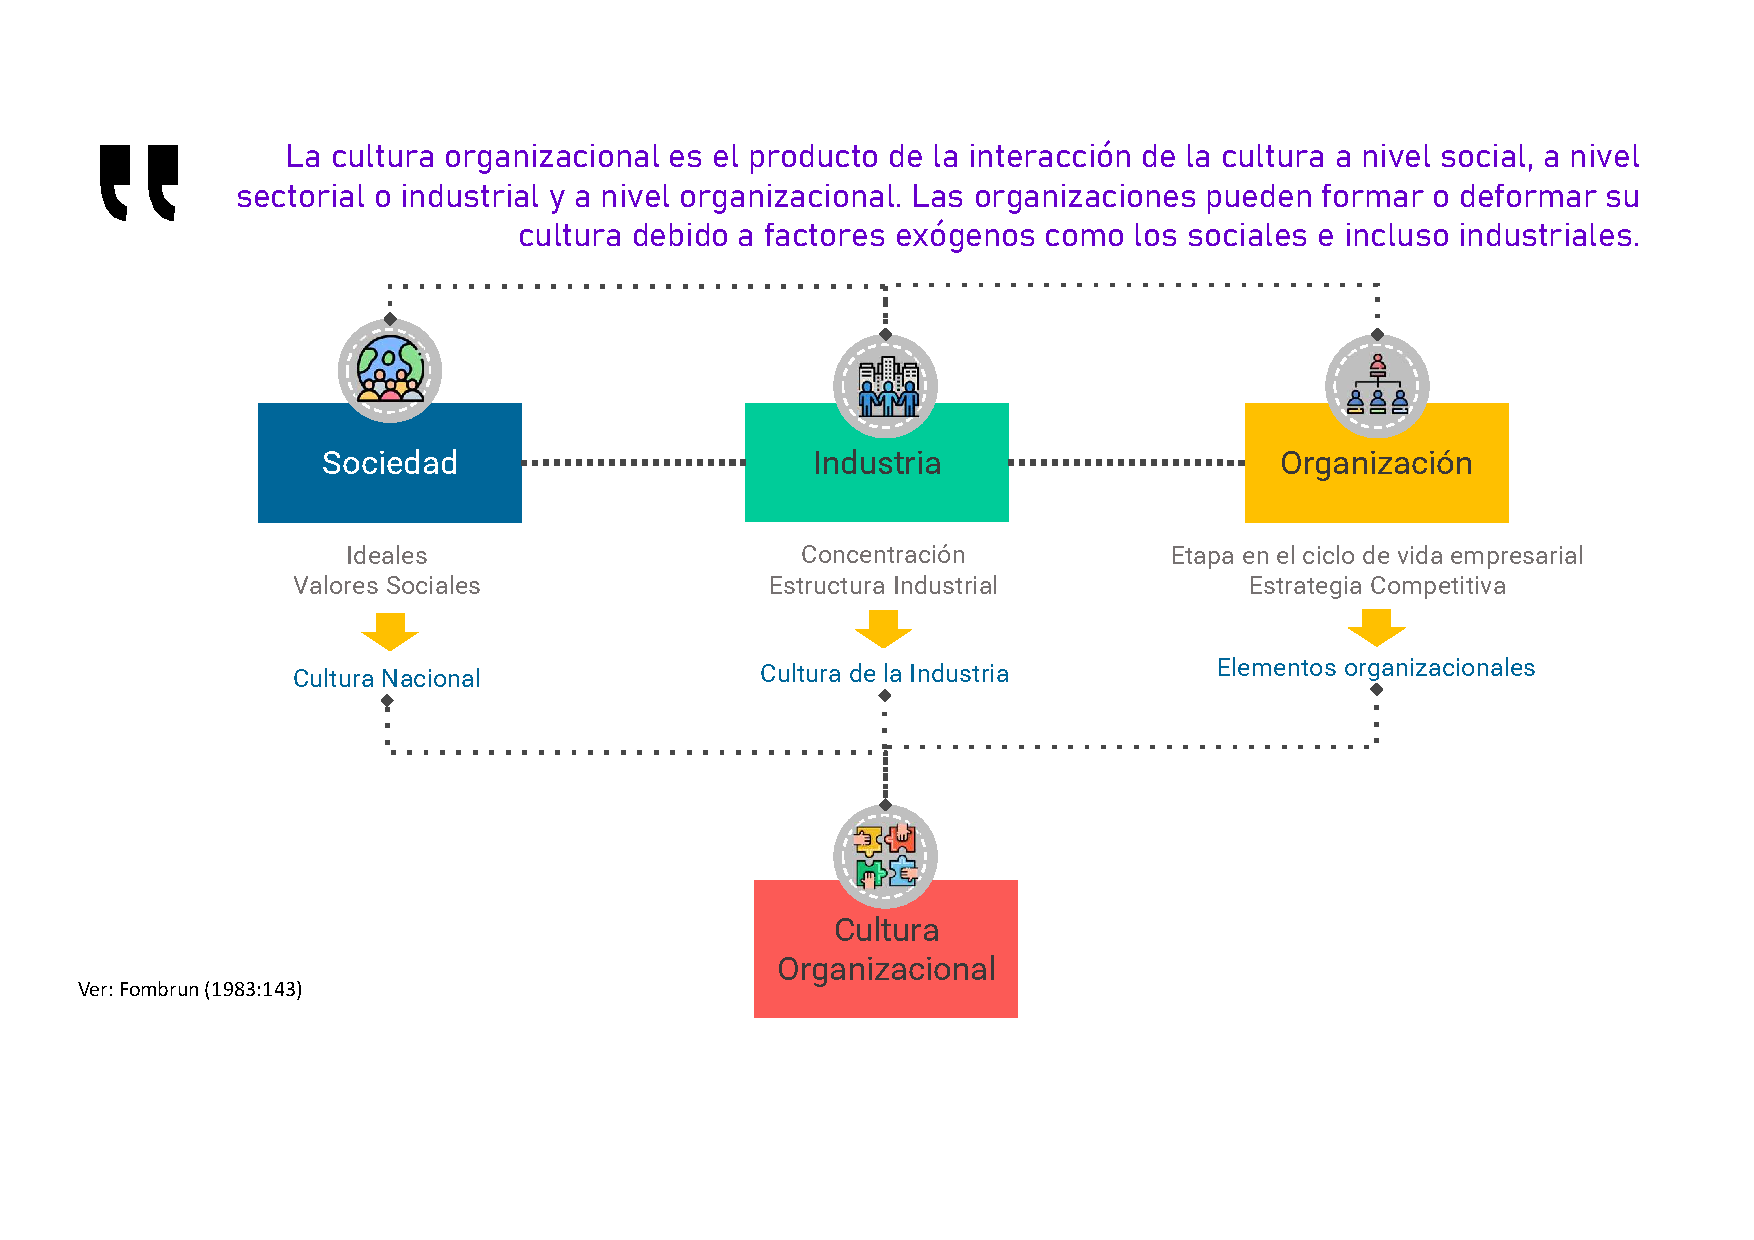
\includegraphics[height=\textheight]{./figures/L6.pdf}
		\end{center}
	\end{frame}

	\begin{frame}{La Cultura como variable}
		\begin{center}
			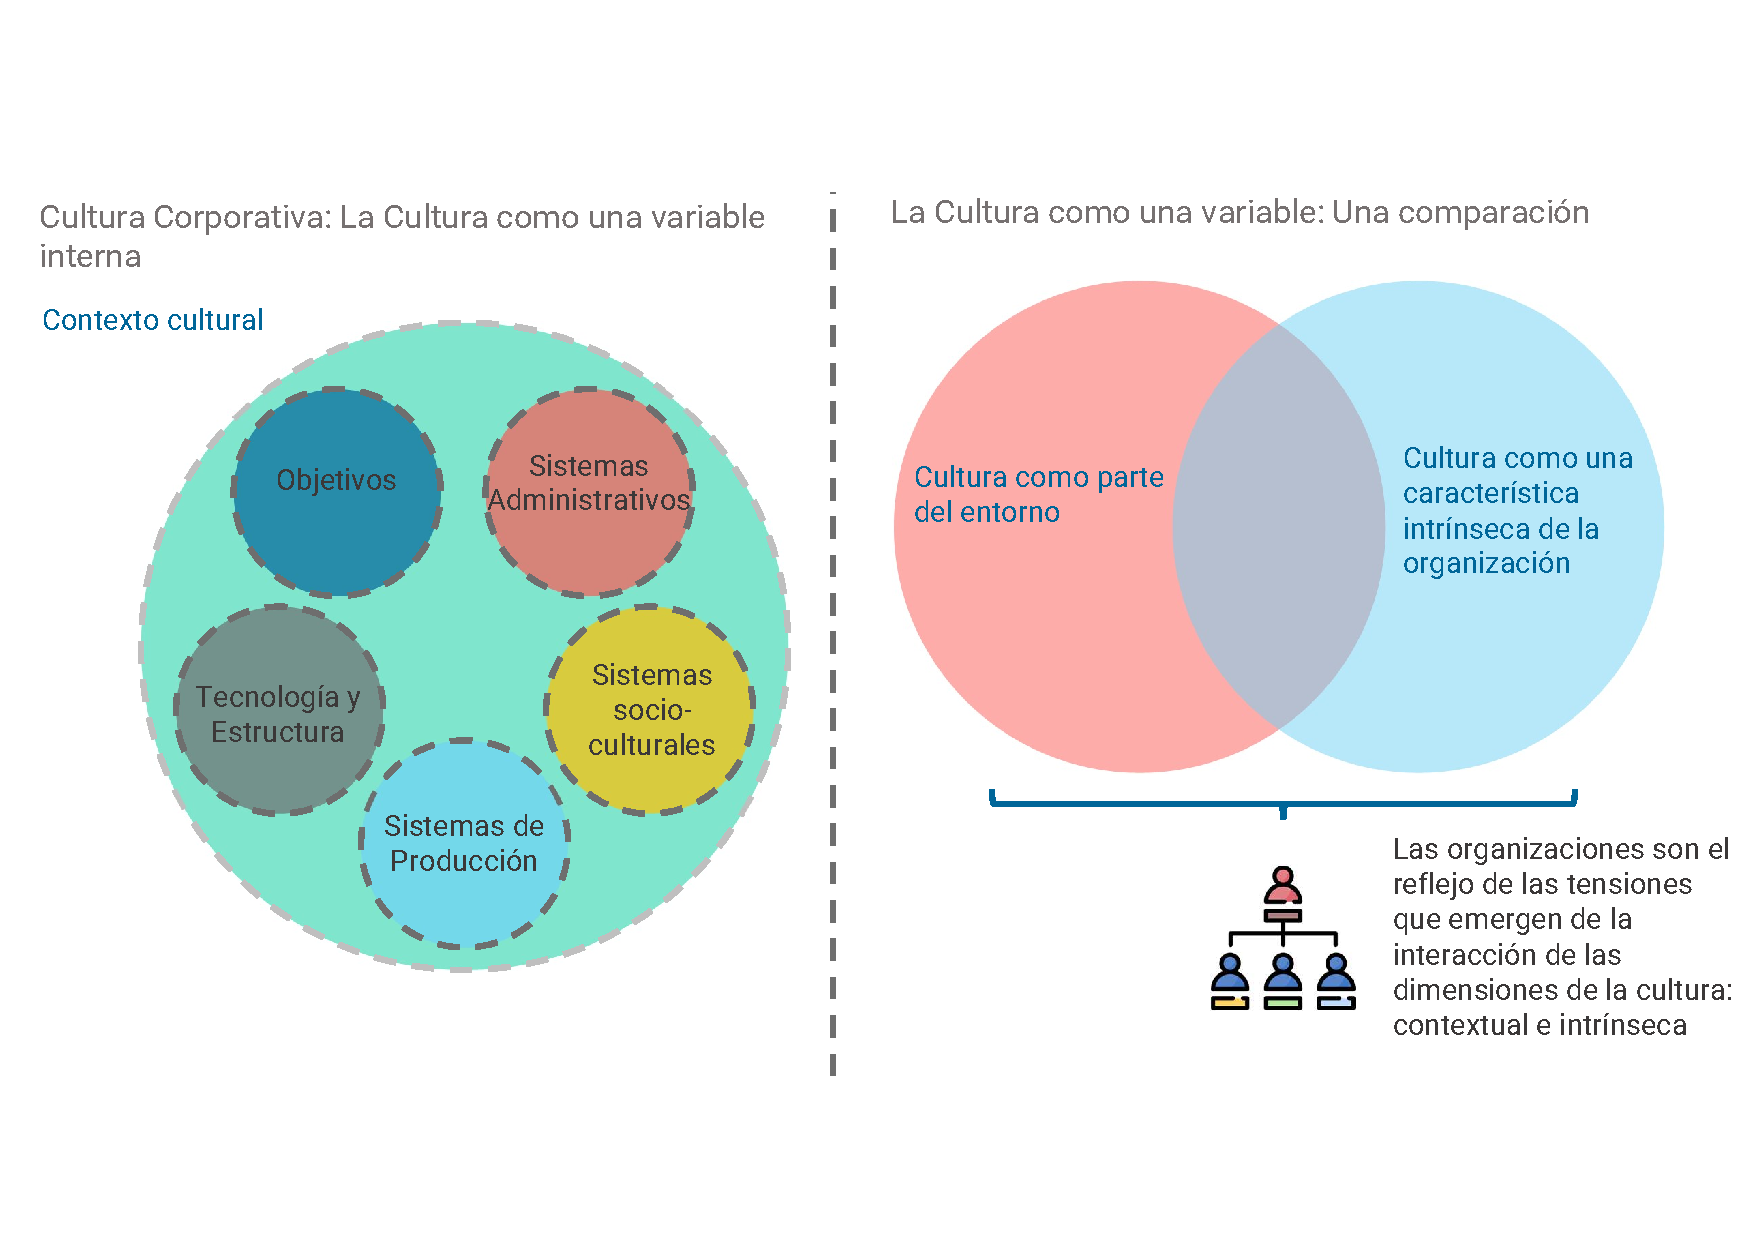
\includegraphics[height=\textheight]{./figures/L7.pdf}
		\end{center}
	\end{frame}

	\begin{frame}{La Cultura como una Metáfora primigenia para conceptualizar a las organizaciones}
		\begin{center}
			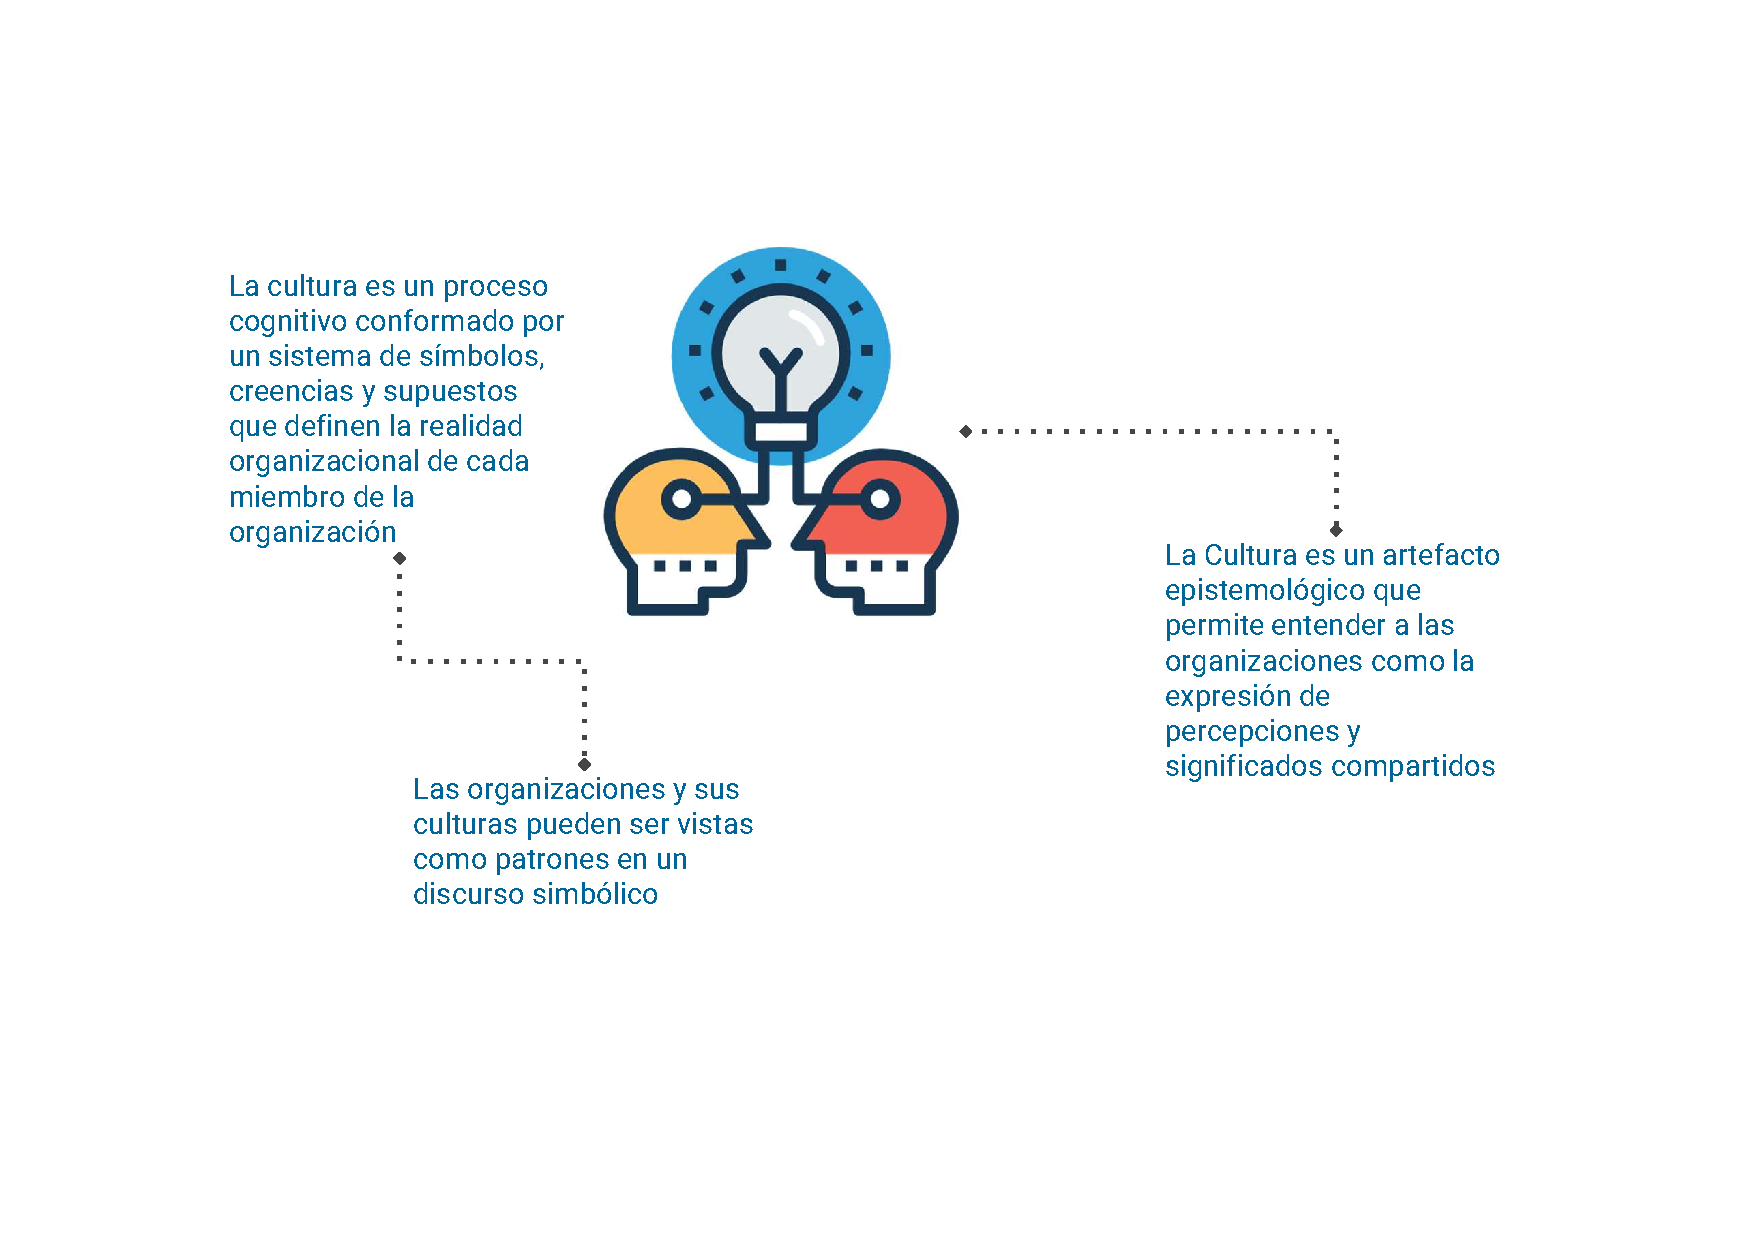
\includegraphics[height=\textheight]{./figures/L8.pdf}
		\end{center}
	\end{frame}

	\begin{frame}{La Cultura como una metáfora primigenia: Una comparación}
		\begin{center}
			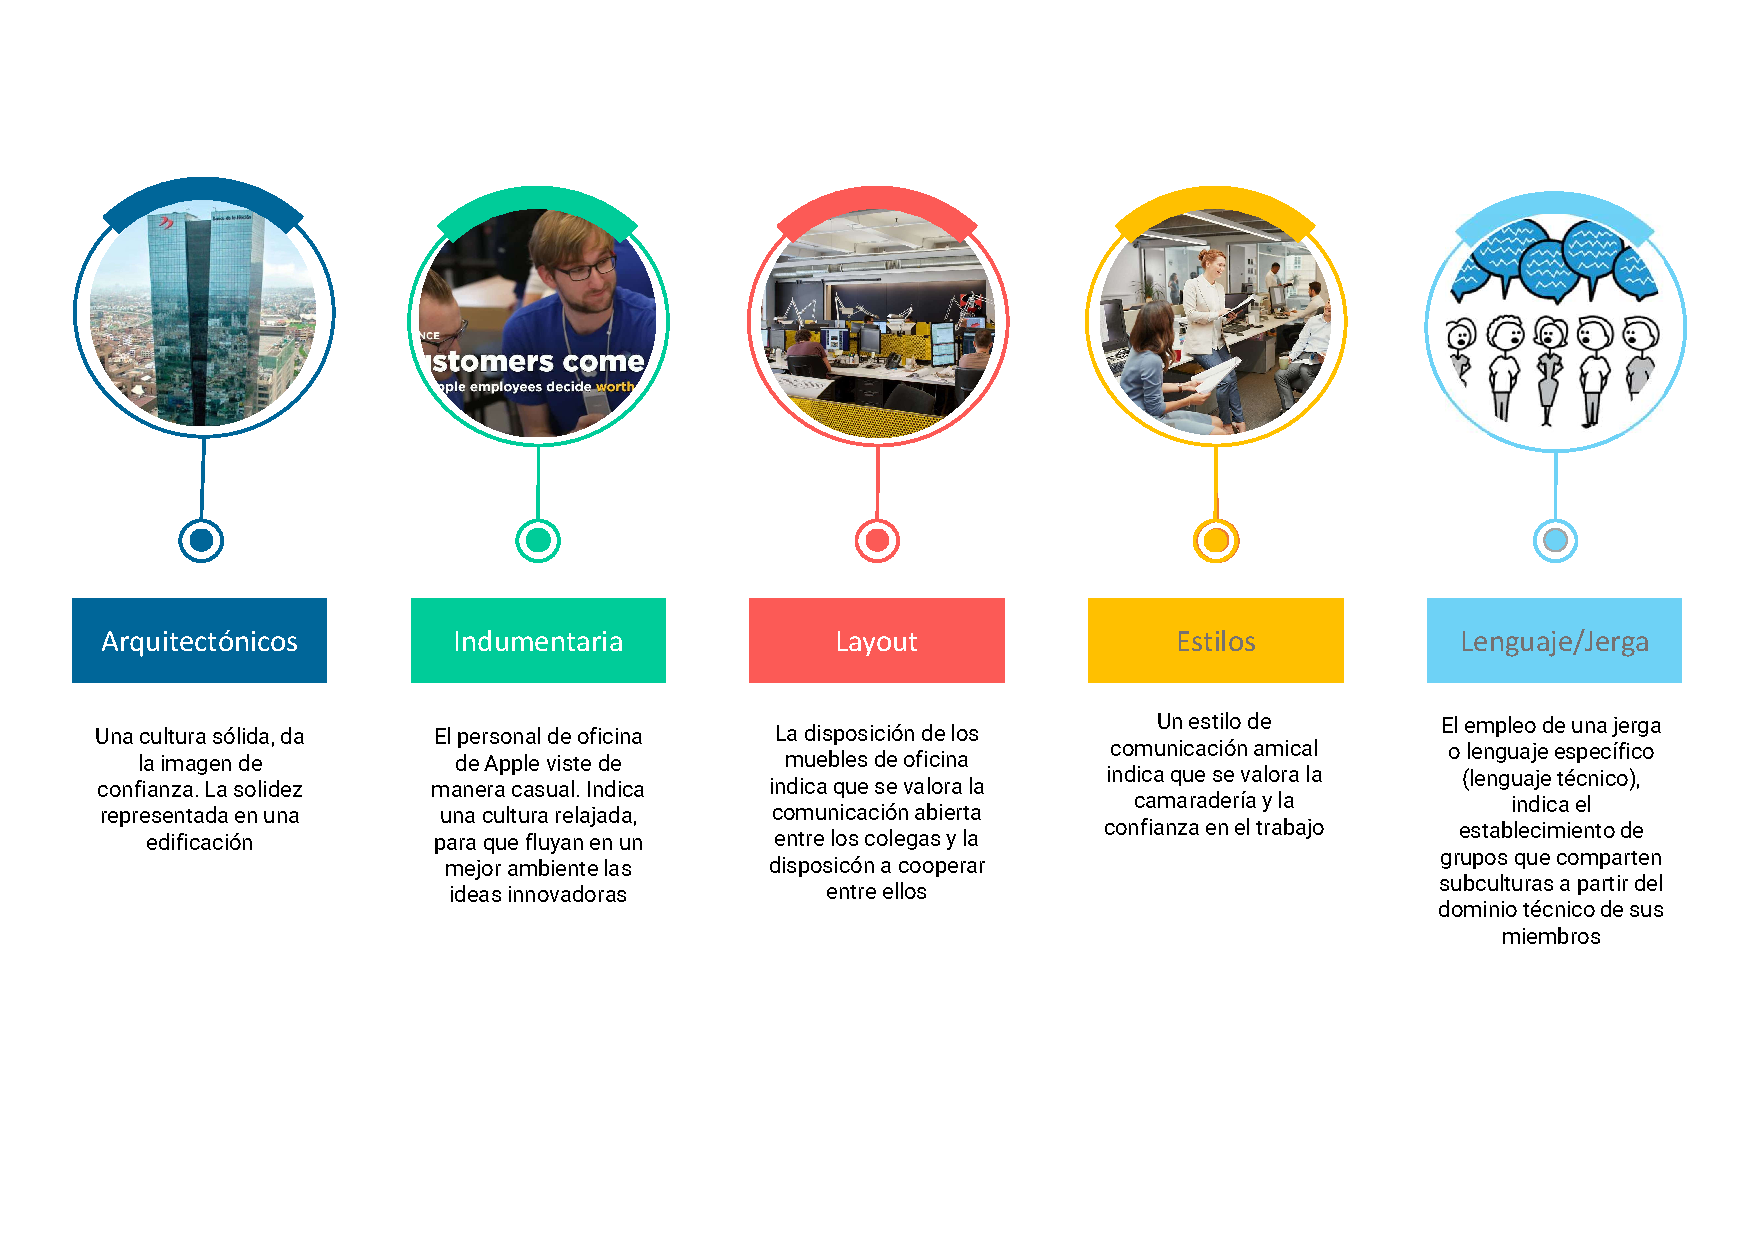
\includegraphics[height=\textheight]{./figures/L9.pdf}
		\end{center}
	\end{frame}

	\begin{frame}{Niveles de análisis: una síntesis}
		\begin{center}
			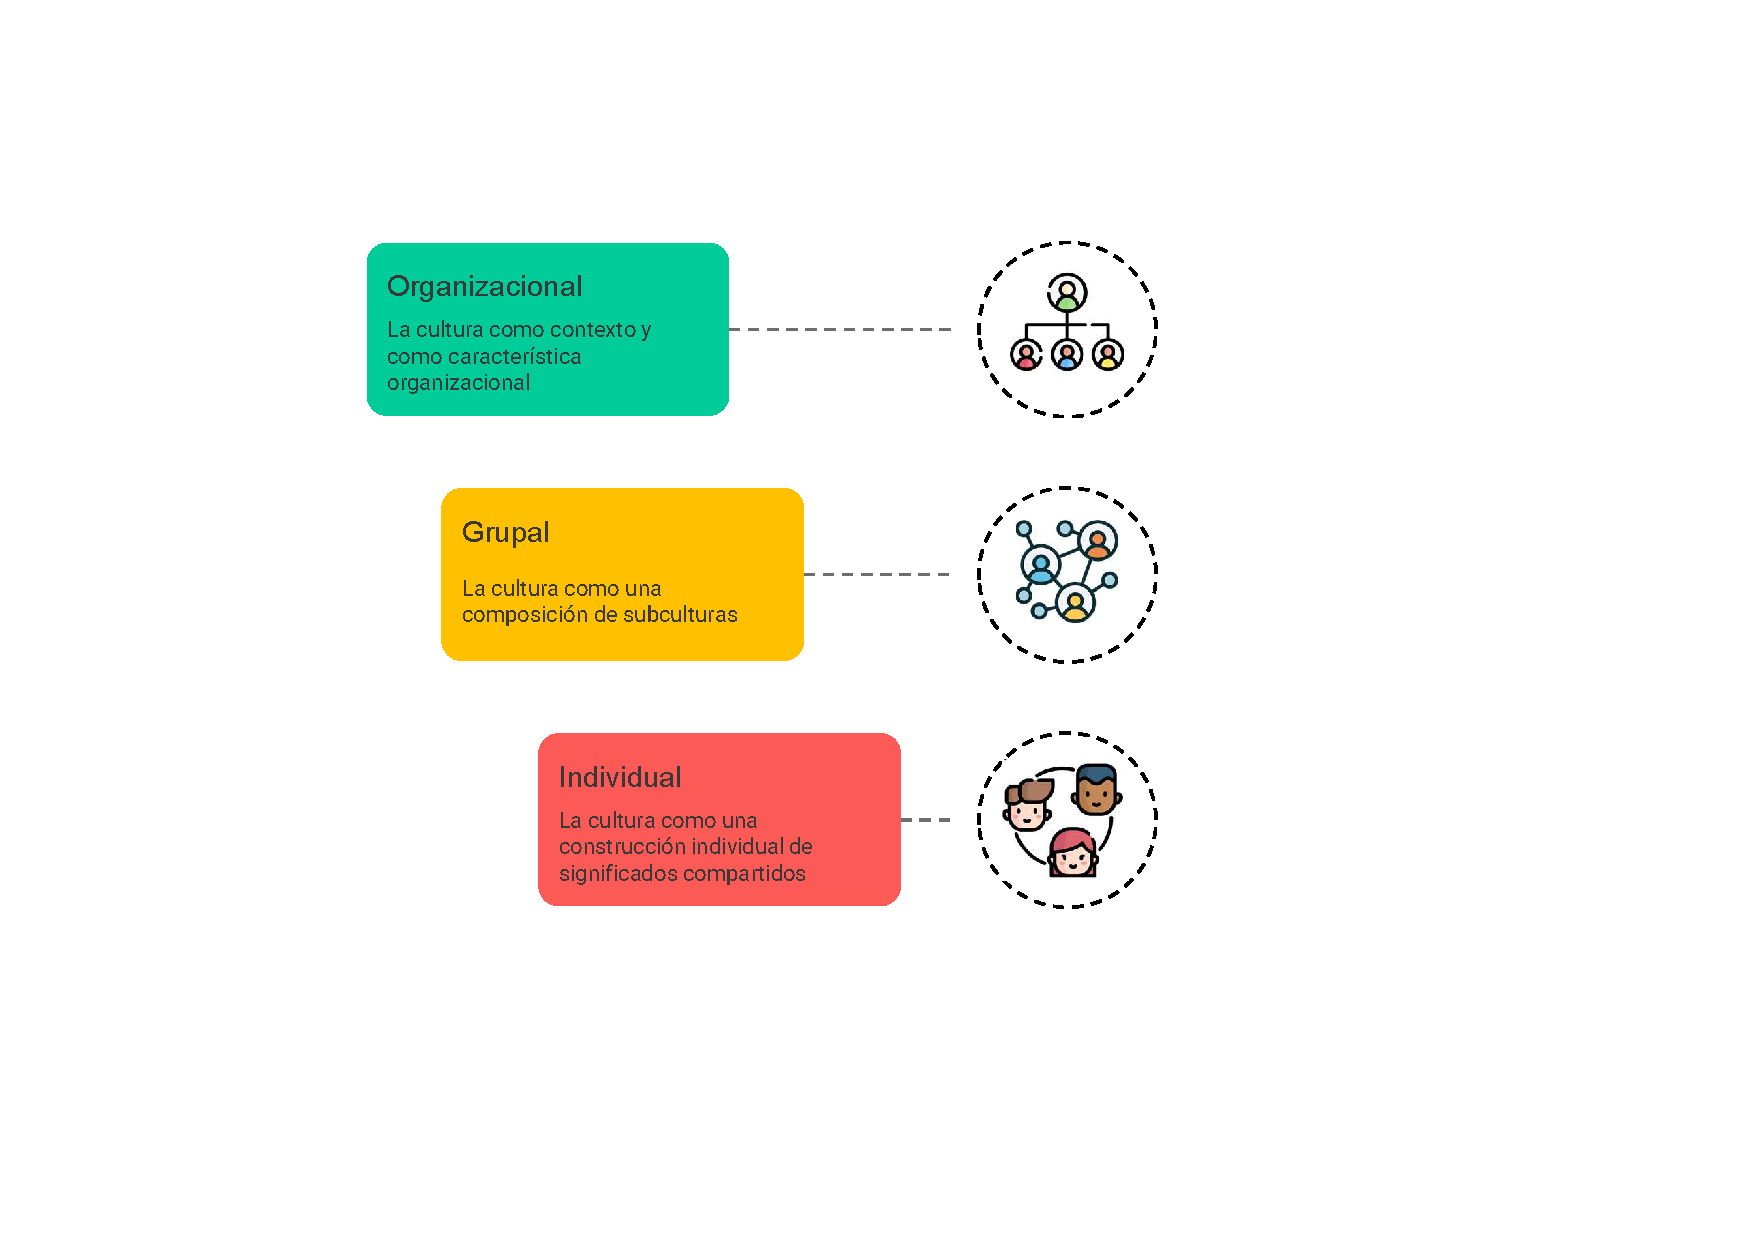
\includegraphics[height=\textheight]{./figures/sintesis.pdf}
		\end{center}
	\end{frame}
	\section{"Cultura Organizacional: una relación dialéctica entre lo deseado y lo vivenciado" (Gentilin, 2019)}
	\begin{frame}
		\begin{center}
			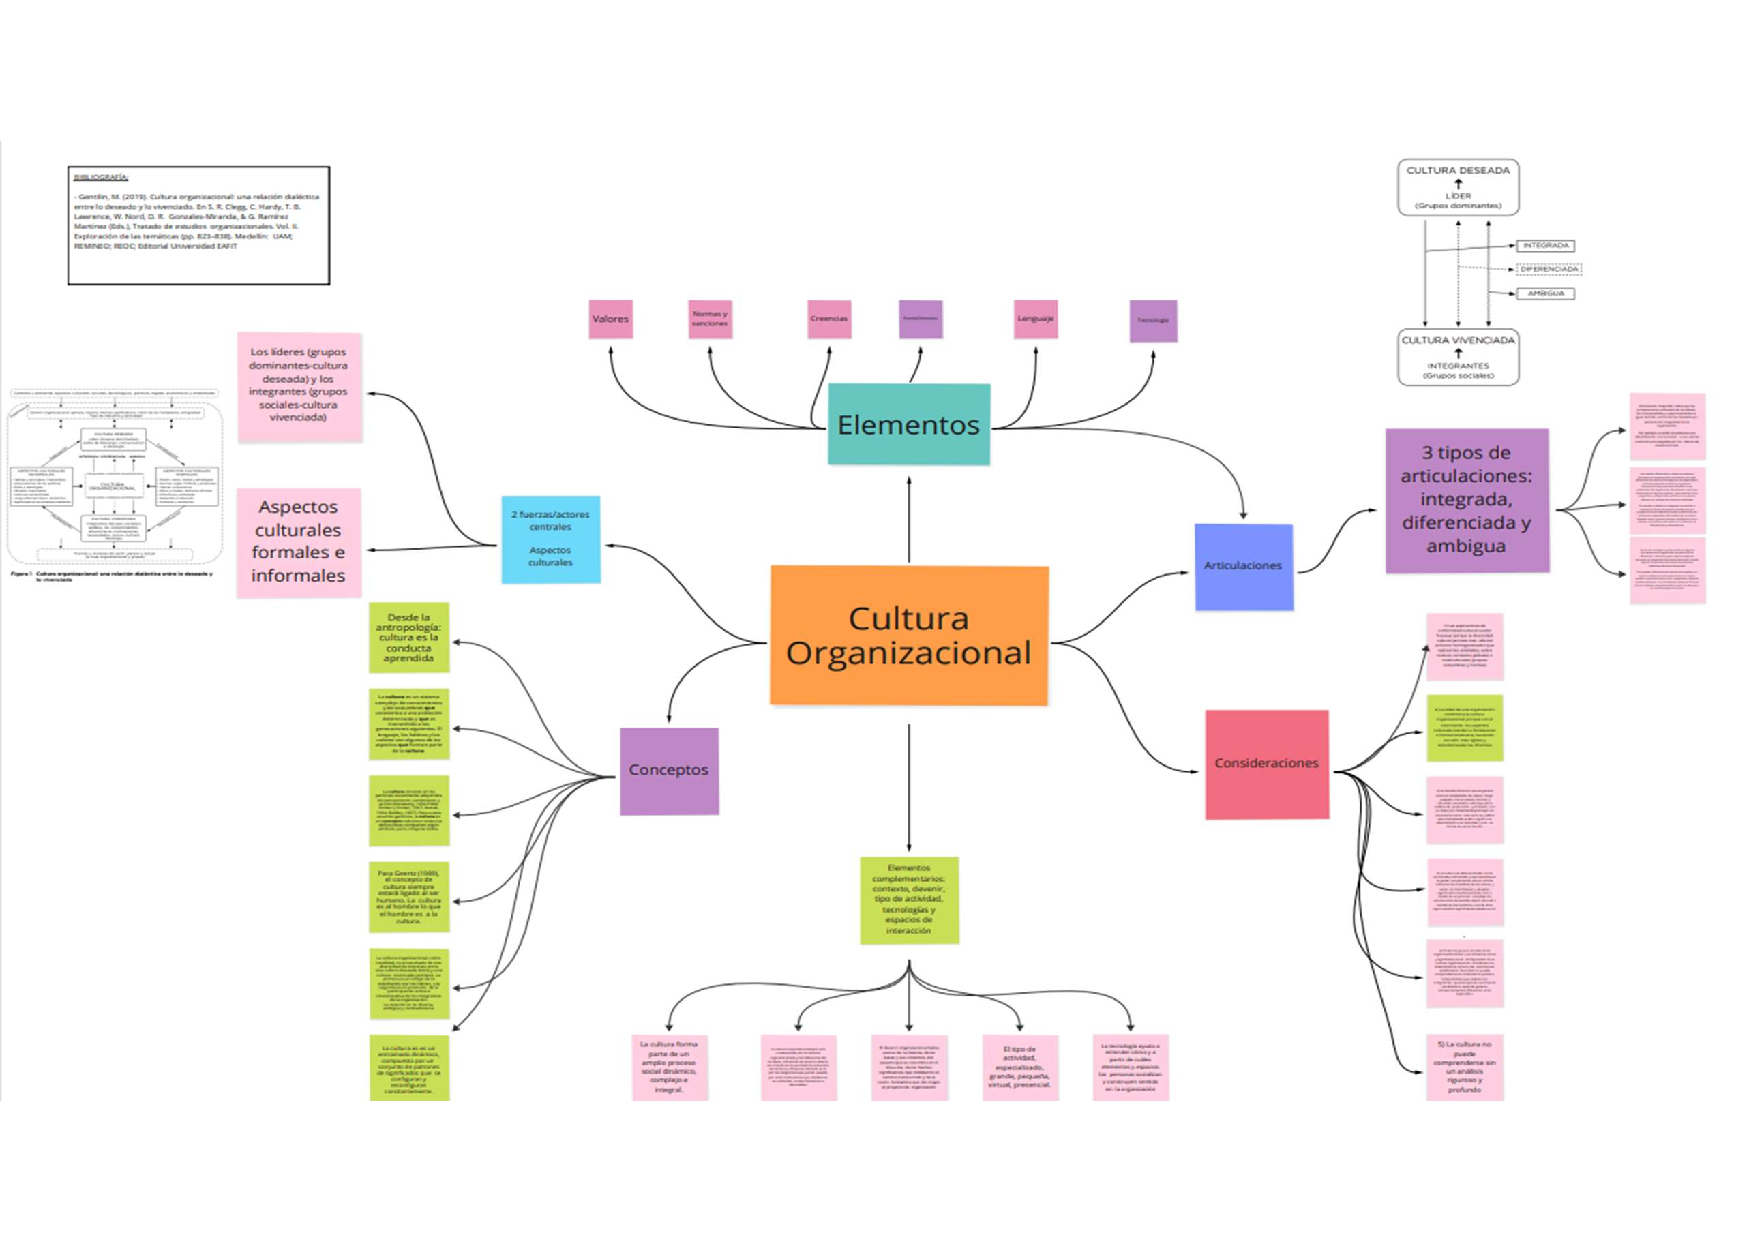
\includegraphics[height=\textheight]{./figures/L10.pdf}
		\end{center}
	\end{frame}

	\begin{frame}{Alineamiento cultural-institucional (Graham et al., 2016)}
		\begin{center}
			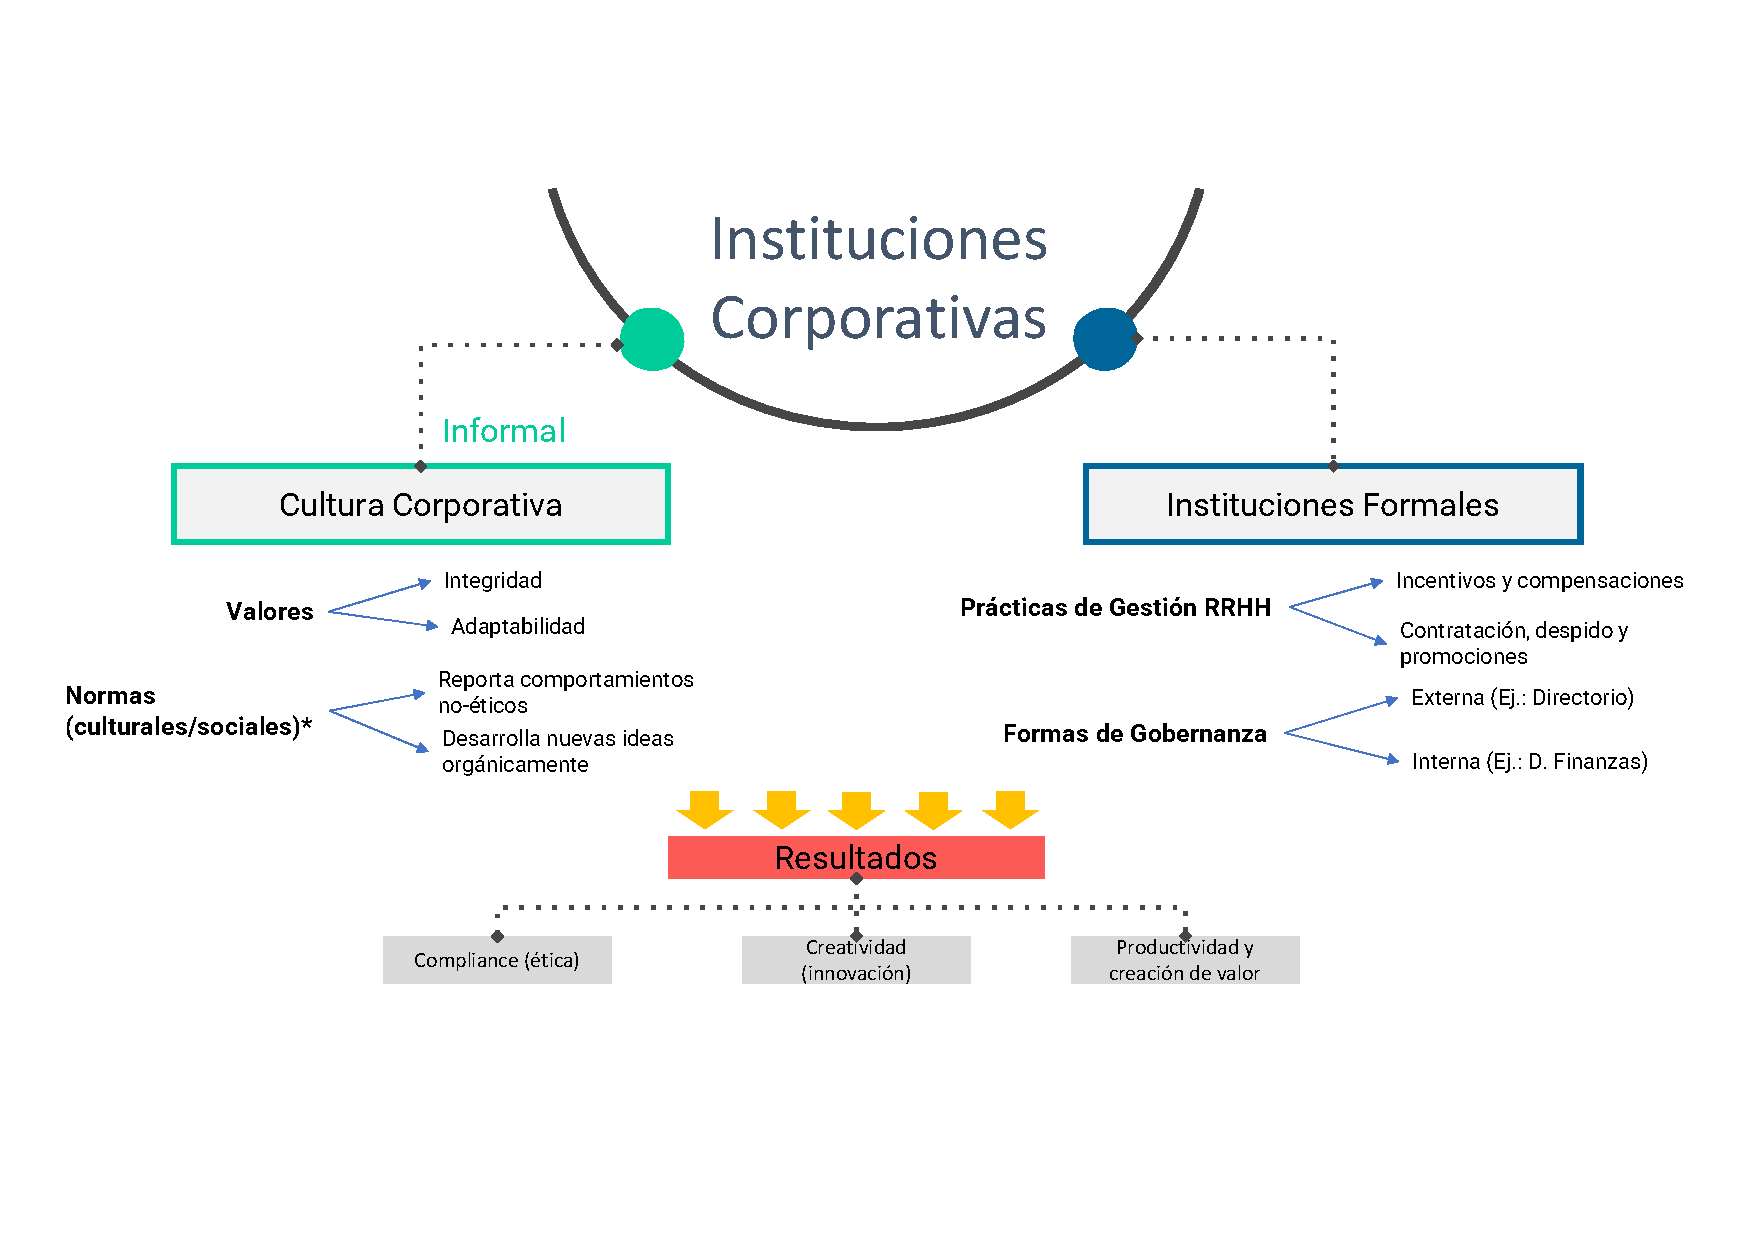
\includegraphics[height=\textheight]{./figures/L11.pdf}
		\end{center}
	\end{frame}
	
	\begin{frame}{Cultura y Estrategia}
		La importancia de la cultura organizacional fue puesta en relevancia en el campo de la gestión y teoría organizacional a partir de la publicación del libro \textbf{En búsqueda de la excelencia}, de Peters y Waterman (1982). Su éxito radicó en el hecho de vincular el logro de los objetivos de la organización con la creación de una cultura organizacional fuerte.
		\end{frame}
	
	\begin{frame}{Discusión}
		\begin{enumerate}
			\item El término de cultura organizacional es un concepto no consensuado conceptualmente. Esta irresolución, que  deriva tanto de diferencias en la concepción, como de la coexistencia de  diversos niveles y métodos de aproximación, conllevan a entendimientos parciales e incompletos de un fenómeno que ante todo, se caracteriza por su complejidad e indeterminación. 
			\item Para Gentilin, los líderes constituyen los grupos dominantes que buscan alcanzar la cultura deseada y los integrantes (grupos sociales-cultura vivenciada). Este supuesto parte de asumir que todos los líderes tendrán las capacidades, visión, para alcanzar esta "cultura deseada". 
			\item Las aspiraciones de uniformidad cultural suelen fracasar porque la diversidad cultural persiste más allá del esfuerzo homogeneizador que realizan las entidades, sobre todo en contextos globales o multiculturales (propias costumbres y normas). 
			\item La cultura se debe entender como construida, mantenida y reproducida por la gente. Ejem: caso de 3 residentes de medicina, uno de ellos logró cambios significativos desde su rol. 
			
		\end{enumerate}
	\end{frame}

	\begin{frame}{Discusión}
		\begin{enumerate}
			\item La cultura no puede comprenderse sin un análisis riguroso y profundo. 
			\item Todos los grupos sociales de la organización tienen una influencia activa y significativa en la configuración de la cultura organizacional. Los líderes no determinan la cultura, tan solo buscan establecerla. 
			\item Pero ésta no puede comprenderse sin entender el proceso interpretativo que realizan los integrantes, quienes ejercen una fuerza modeladora capaz de generar comportamientos diferentes a los esperados. 
		\end{enumerate}
	\end{frame}
	\begin{frame}{Cultura Organizacional hoy}
		\begin{center}
			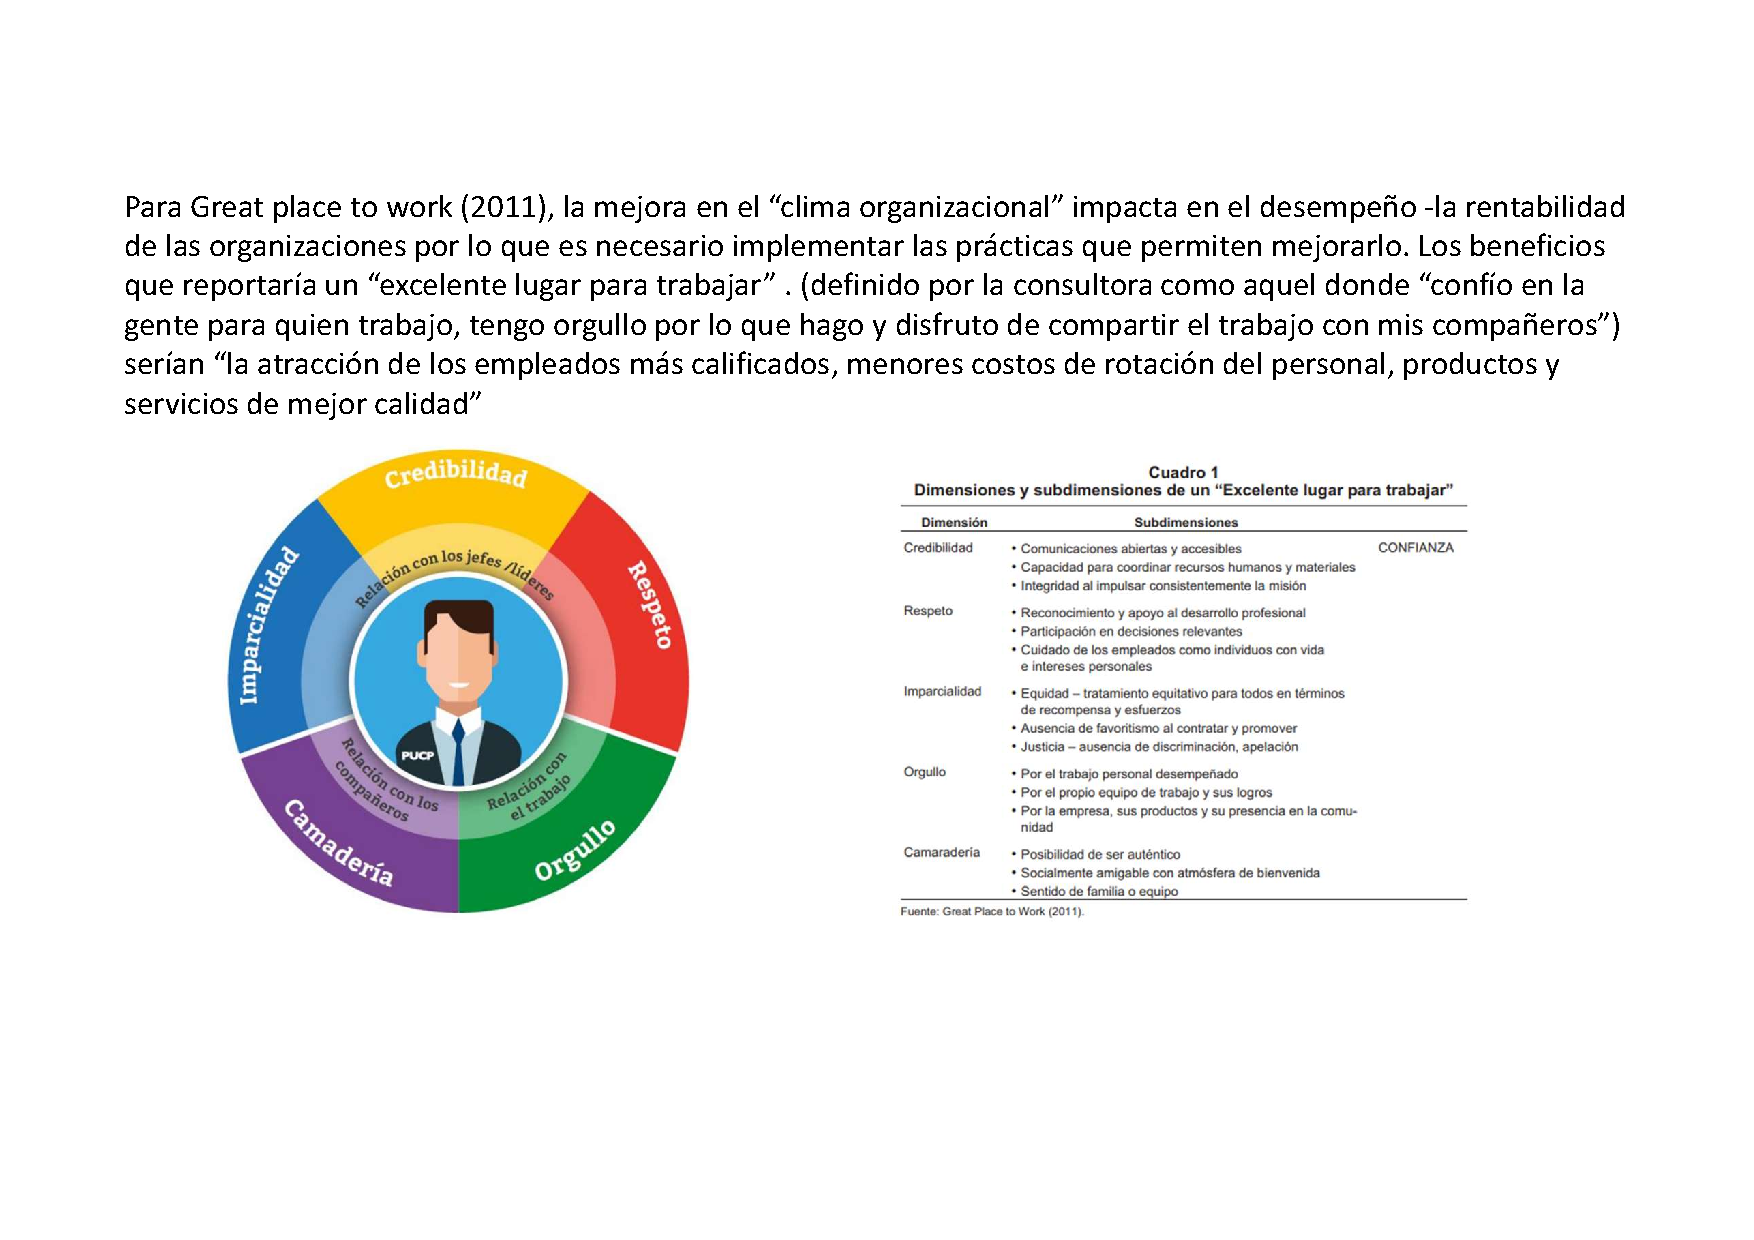
\includegraphics[height=\textheight]{./figures/L13.pdf}
		\end{center}
	\end{frame}
	
	\begin{frame}{Cultura Organizacional hoy}
		\begin{center}
			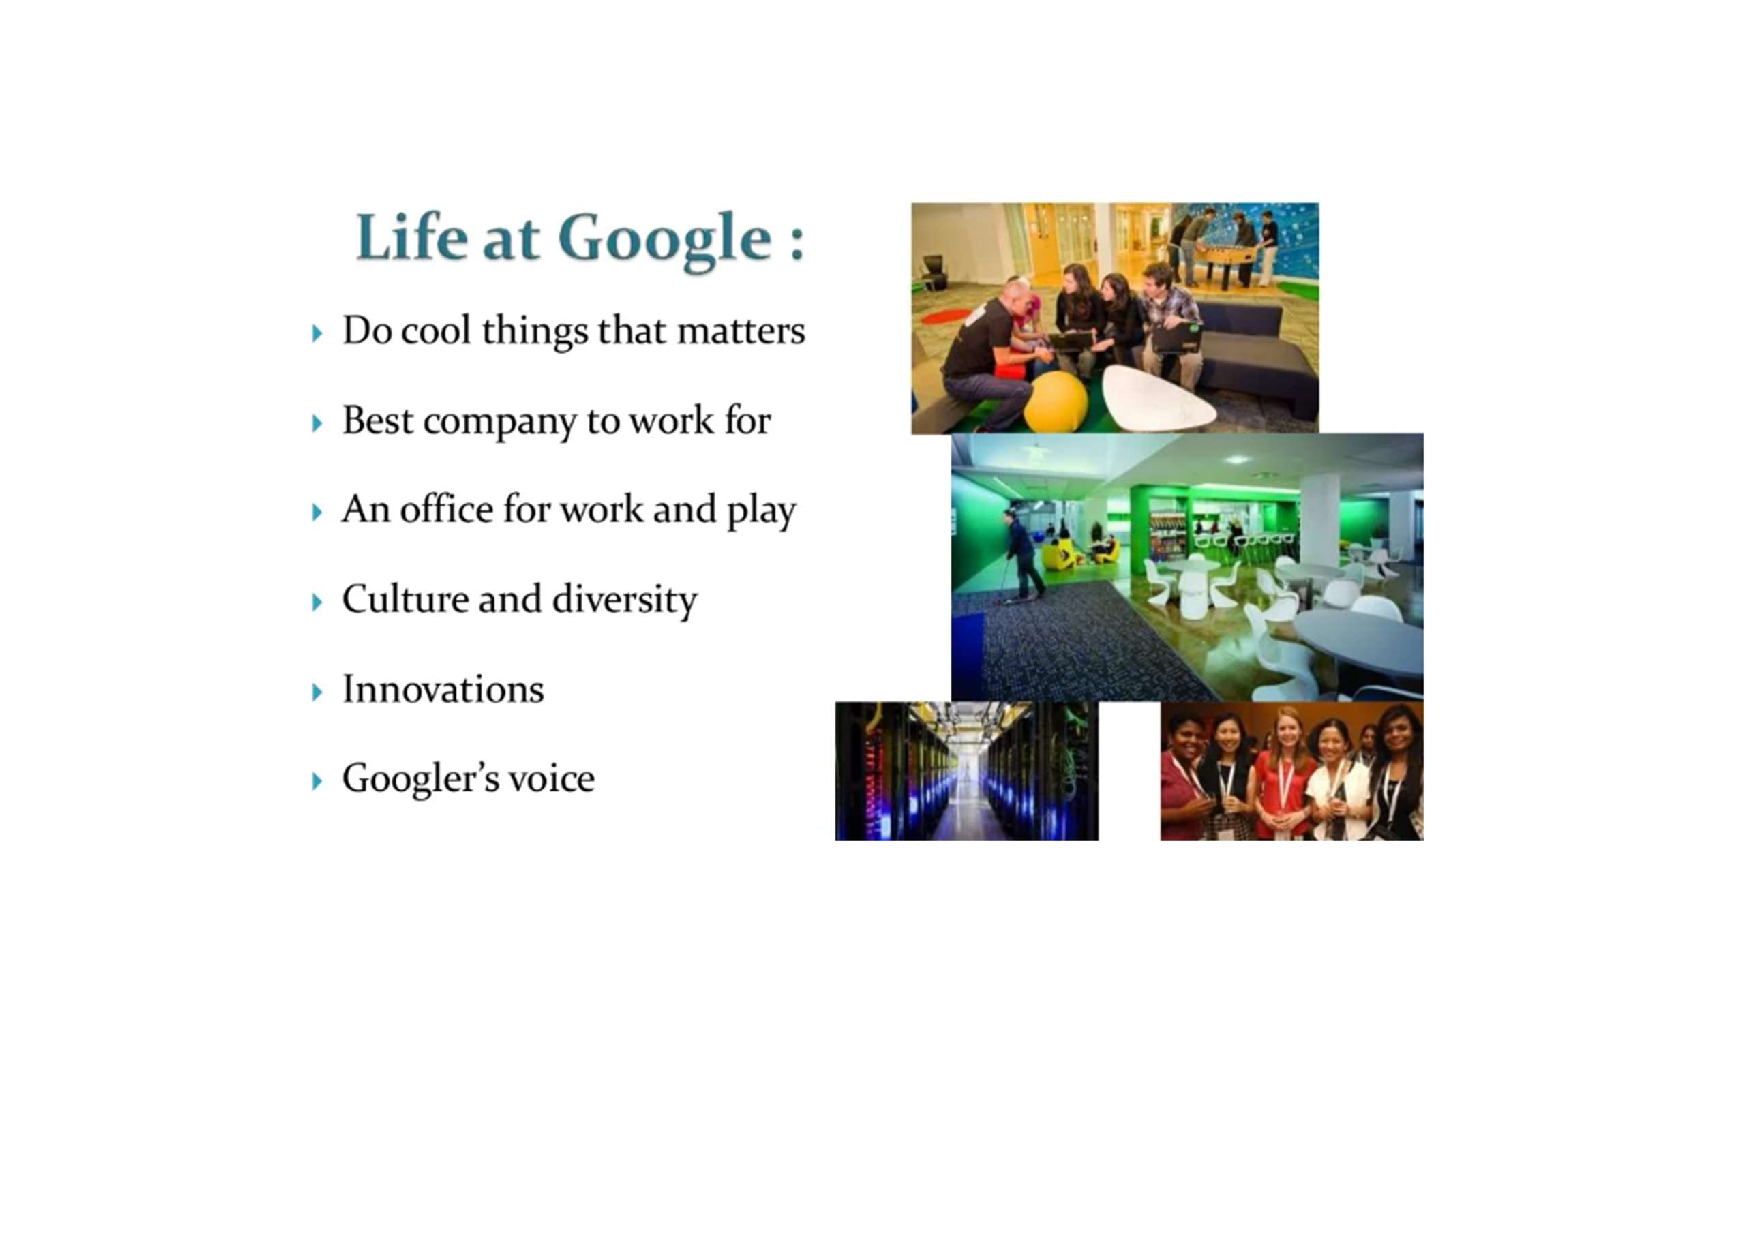
\includegraphics[height=\textheight]{./figures/L14.pdf}
		\end{center}
	\end{frame}

	\begin{frame}{Cultura Organizacional hoy}
		\begin{center}
			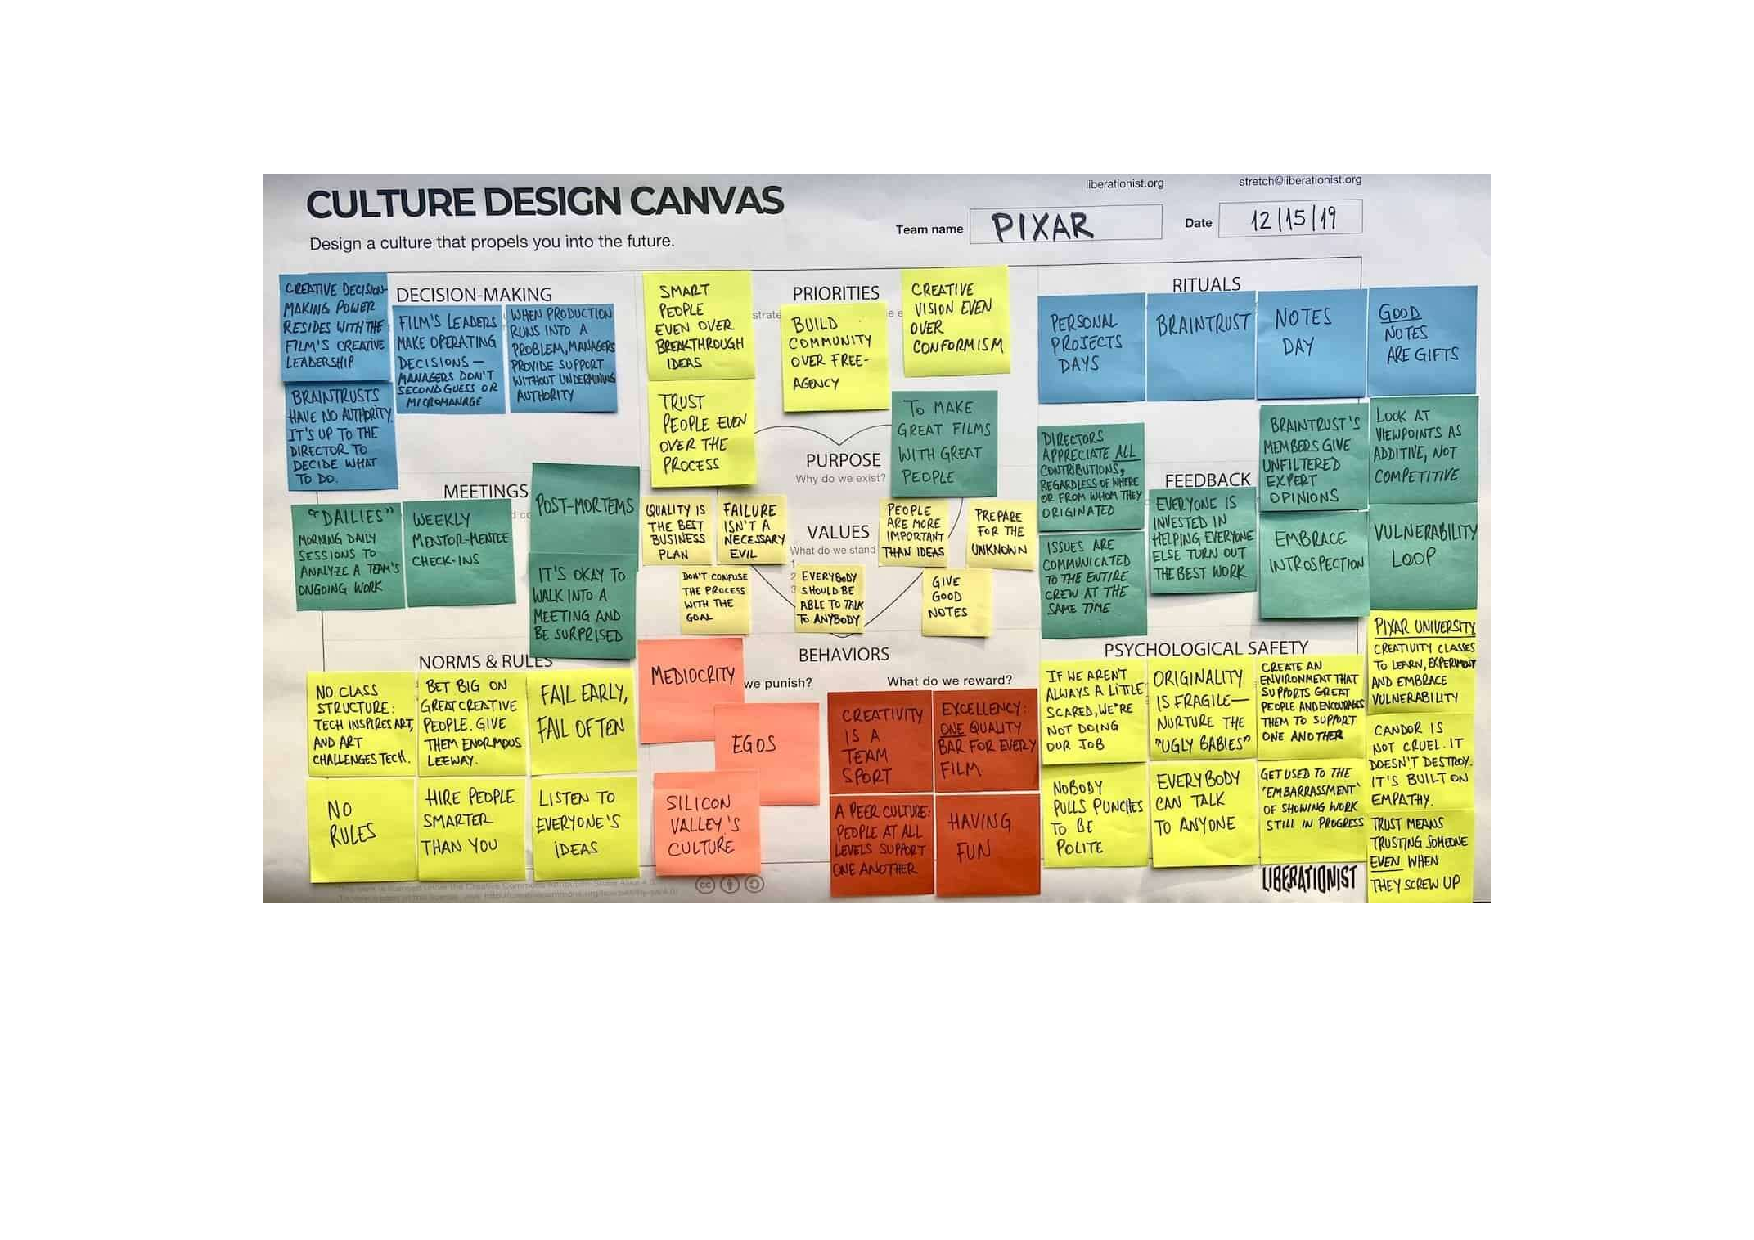
\includegraphics[height=\textheight]{./figures/L15.pdf}
		\end{center}
	\end{frame}

	\begin{frame}{Cultura Organizacional hoy}
		\begin{center}
			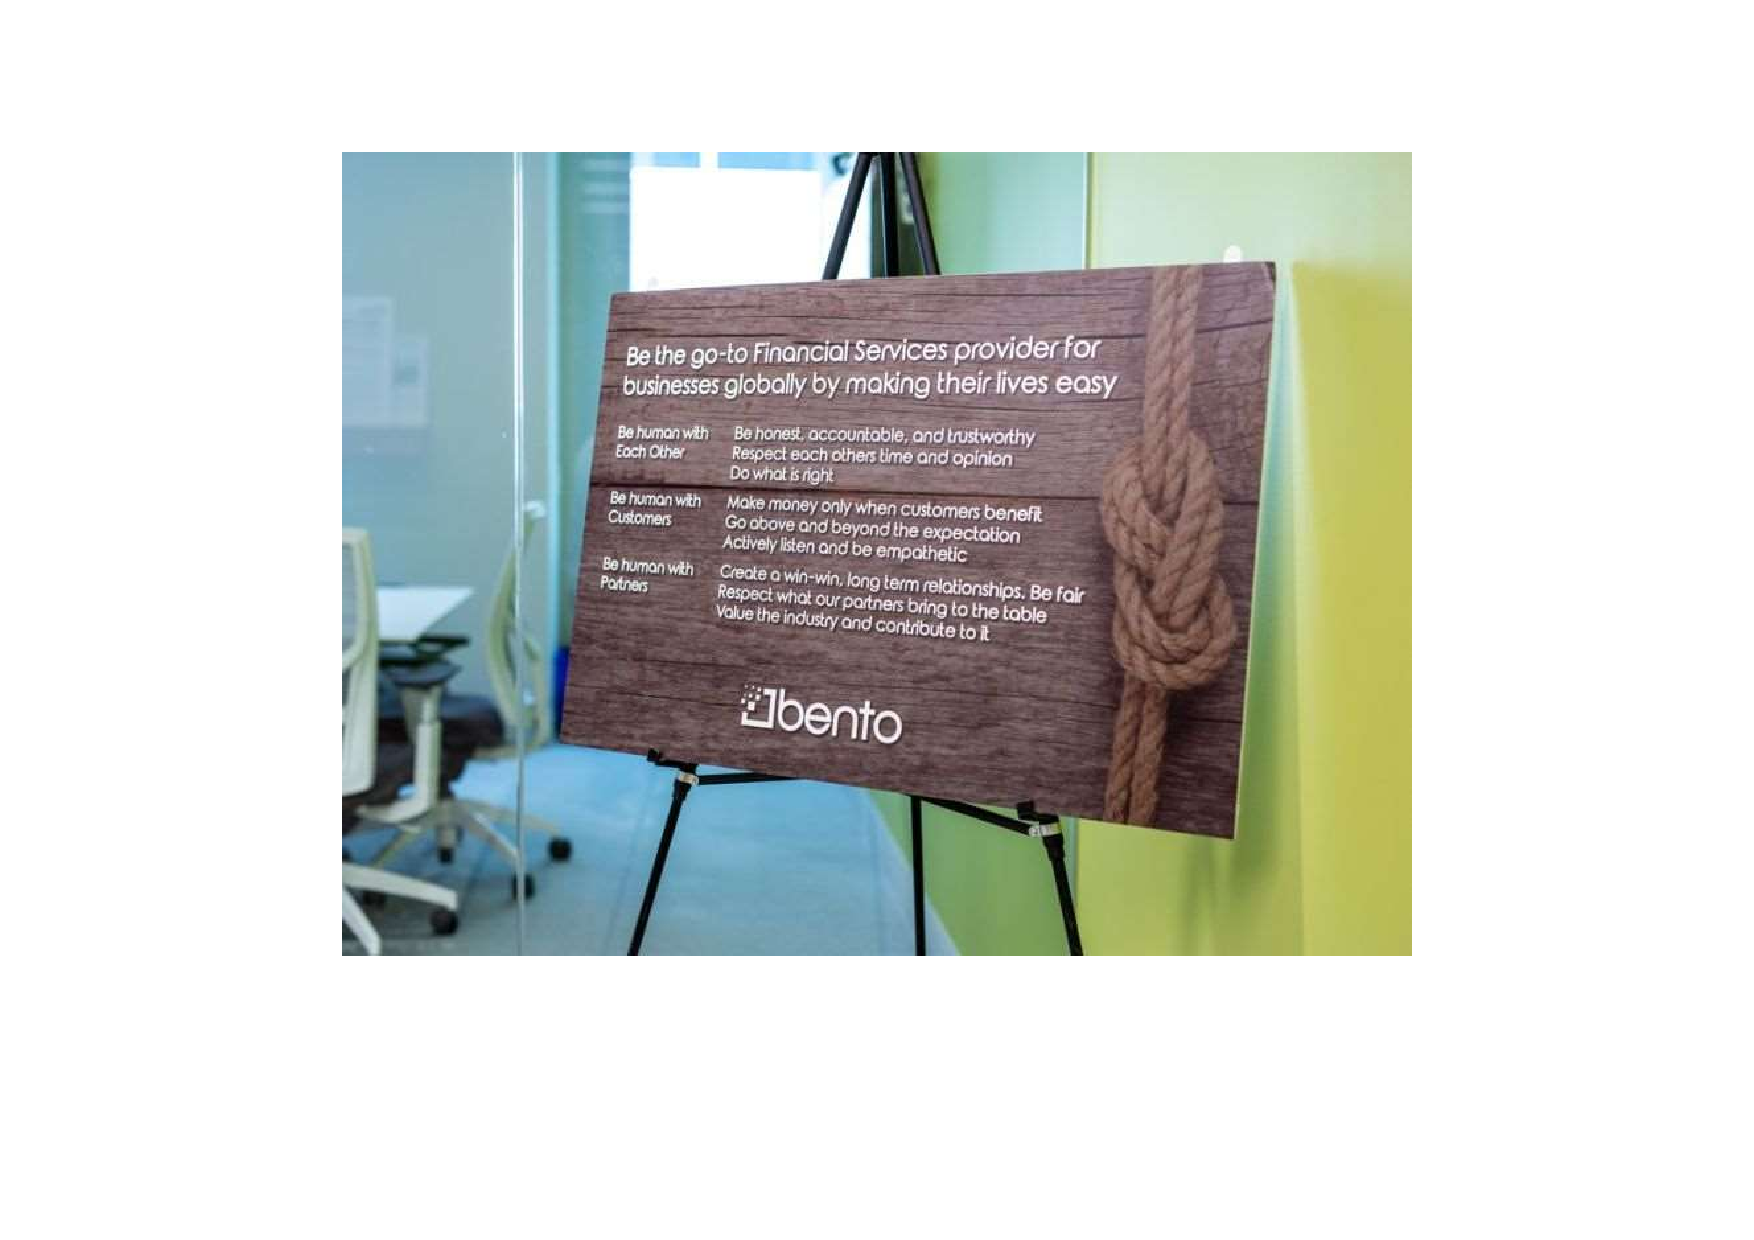
\includegraphics[height=\textheight]{./figures/L16.pdf}
		\end{center}
	\end{frame}

	\begin{frame}{Cultura Organizacional hoy}
		\begin{center}
			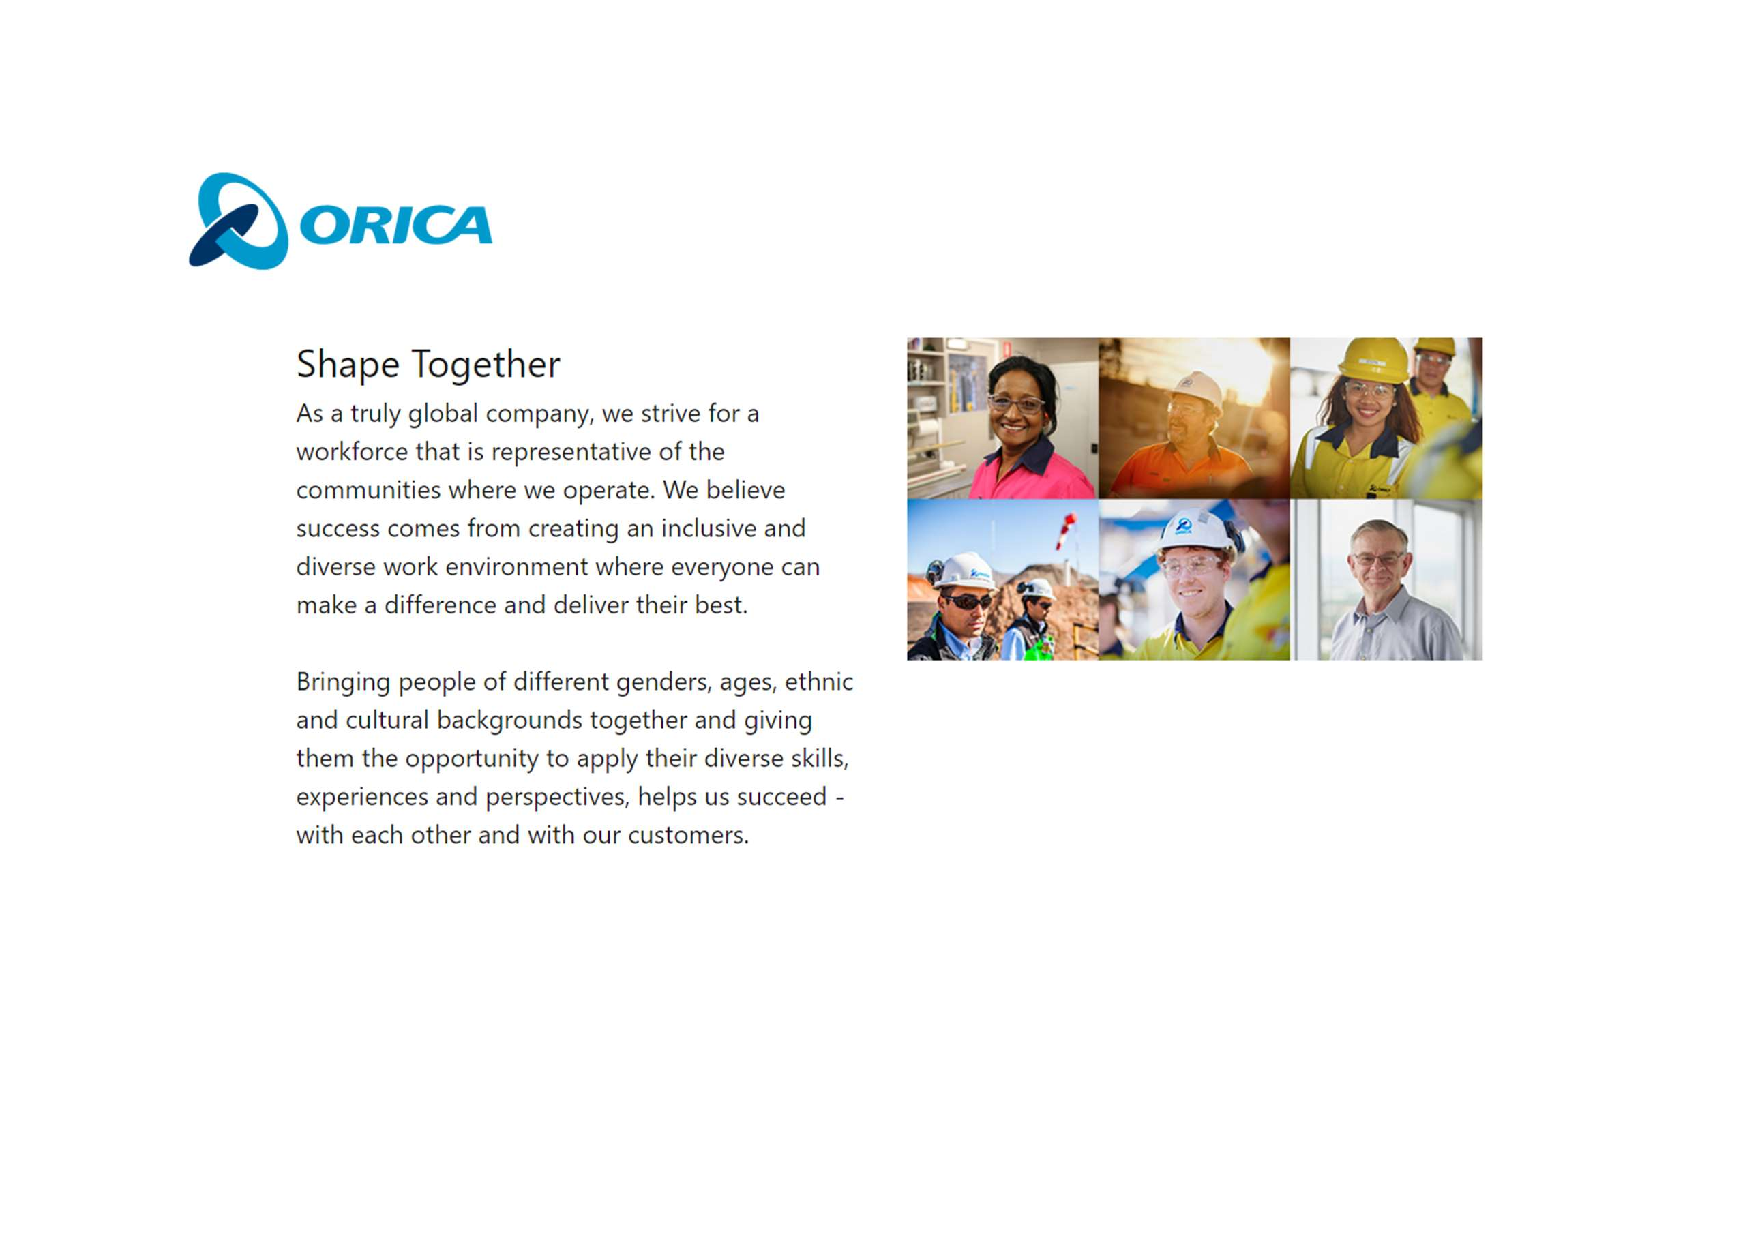
\includegraphics[height=\textheight]{./figures/L17.pdf}
		\end{center}
	\end{frame}
\end{document}